% this file is encoded in utf-8
% v1.7

\documentclass[12pt, a4paper]{ntust_report} 

\usepackage{fontspec}		%加這個就可以設定字體 
\usepackage{xeCJK}       	%讓中英文字體分開設置 
\usepackage{indentfirst}  	%首行縮排
\usepackage[table,xcdraw]{xcolor}  % 表格顏色
\usepackage{pdfpages}		%用來插入推薦書與審定書,詳見ntust_frontpages.tex
\usepackage{algorithm}		% 演算法用
\usepackage{algorithmic}
\usepackage{diagbox}
\usepackage{rotating}

\renewcommand{\algorithmicrequire}{ \textbf{Input:}} %Use Input in the format of Algorithm
\renewcommand{\algorithmicensure}{ \textbf{Output:}} %UseOutput in the format of Algorithm

\setmainfont[Mapping=tex-text]{Times New Roman}   %設定主要字型,也就是英文字型 
\setCJKmainfont{標楷體}     				%設定中文字型 
\XeTeXlinebreaklocale "zh"				%這兩行一定要加,中文才能自動換行 
\XeTeXlinebreakskip = 0pt plus 1pt		%這兩行一定要加,中文才能自動換行

\setCJKfamilyfont{zero}{新細明體}			%中華民國的108的0
\newcommand{\zero}{\CJKfamily{zero}}
\setCJKfamilyfont{bai}{標楷體}
\newcommand{\bai}{\CJKfamily{bai}}
\newcommand{\tabincell}[2]{\begin{tabular}{@{}#1@{}}#2\end{tabular}}





% 除非校方修改了論文格式 (margins, header, footer, 浮水印)
% 或者需要增加所用的 LaTeX 套件,
% 或者要改預設中文字型、編碼
% 否則毋須修改本檔內容
% 論文撰寫,請修改以 my_  開頭檔名的各檔案



\usepackage{titletoc}
\usepackage[nospace]{cite}  % for smart citation
\usepackage{geometry}  % for easy margin settings
\usepackage{subfigure}  % for subfigure
\usepackage{multirow}
%\usepackage[dvipdfm]{graphicx}  % for graphic   using eps
\usepackage{graphicx}  % for graphic   using eps

%\usepackage{epstopdf} % 當使用pdflatex時打開,如使用latex則不需開啟,此功能為將xxx.eps 自動判讀為XXX.pdf

%\usepackage{subfig} 
\usepackage{algorithmic}  %演算法使用
\usepackage{algorithm}

%
% margins setting
\geometry{verbose,a4paper,tmargin=3.5cm,bmargin=2cm,lmargin=3cm,rmargin=3cm}
%
\usepackage{amsmath} % 各式 AMS 數學功能
\usepackage{amssymb} % 各式 AMS 數學符號
\usepackage{mathrsfs} %草寫體數學符號,在數學模式裡用 \mathscr{E} 得草寫 E
\usepackage{listings} % 程式列表套件
%
% listing setting
\lstset{breaklines=true,% 過長的程式行可斷行
extendedchars=false,% 中文處理不需要 extendedchars
texcl=true,% 中文註解需要有 TeX 處理過的 comment line, 所以設成 true
comment=[l]\%\%,% 以雙「百分號」做為程式中文註解的起頭標記,配合 MATLAB
basicstyle=\small,% 小號字體, 約 10 pt 大小
commentstyle=\upshape,% 預設是斜體字,會影響註解裏的英文,改用正體
%language=Octave % 會將一些 octave 指令以粗體顯示
}

\usepackage{url} % 在文稿中引用網址,可以用 \url{http://www.ntust.edu.tw} 方式

% 插圖套件 graphicx
% 使用者工作流程是用 pdftex 還是 latex + dvipdfmx?
% 視情況而有不同的參數
% 這裡作自動判斷
% 參考自
% http://www.tex.ac.uk/cgi-bin/texfaq2html?label=ifpdf
%\newcommand\mydvipdfmxflow{dvipdfmx}
%\newcommand\mypdftexflow{pdftex}
%
%\ifx\pdfoutput\undefined
%  % not running pdftex
%  \usepackage[dvipdfm]{graphicx}
%  \newcommand\myworkflow{dvipdfmx}  % set the flag for hyperref
%\else
%  \ifx\pdfoutput\relax
%    % not running pdftex
%    \usepackage[dvipdfm]{graphicx}
%    \newcommand\myworkflow{dvipdfmx}  % set the flag
%  \else
%    % running pdftex, with...
%    \ifnum\pdfoutput>0
%      % ... PDF output
%      \usepackage[pdftex]{graphicx}
%      \newcommand\myworkflow{pdftex}  % set the flag
%    \else
%      %...DVI output
%      \usepackage[dvipdfm]{graphicx}
%      \newcommand\myworkflow{dvipdfmx}  % set the flag
%    \fi
%  \fi
%\fi

\usepackage{fancyhdr}  % 借用增強功能型 header 套件來擺放浮水印 
% (佔用了 central header)
% 不需要浮水印的使用者仍可利用此套件,產生所需的 header, footer
%
% 啟動 fancy header/footer 套件
\pagestyle{fancy}
\fancyhead{}  % reset left, central, right header to empty
\fancyfoot[C]{\thepage} %中間 footer 擺放頁碼
\renewcommand{\headrulewidth}{0pt} % header 的直線; 0pt 則無線

% 如果不需要任何浮水印,則請把下列介於 >>> 與 <<< 之間
% 的文字行關掉 (行首加上百分號)
%% 浮水印 >>> 
%7/23
%
% this file is encoded in utf-8
% v1.7
% 如果浮水印不是全篇需要,請把下列介於 >>> 與 <<<
% 的「全篇浮水印專用碼」關掉 (行首加百分號)
% 參考自 Keith Reckdahl 寫的 "Using Imported Graphics in LATEX2e" (epslatex.pdf) p.39
% 如果只有特定頁需要浮水印
% 則依該頁屬性使用下列之一的命令 
% 普通頁命令 \thispagestyle{WaterMarkPage}
% plain 頁命令 \thispagestyle{PlainWaterMarkPage}
% empty 頁命令 \thispagestyle{EmptyWaterMarkPage}


% 將重複使用的浮水印章
% 圖檔是 my_watermark.xxx
% 副檔名可以不加,可以是 latex 系統能處裡的任何格式:pdf, gif, png, jpg, eps, ...
% 某些圖檔格式在某些工作流程可能需要作前置處裡。
% 例如,pdflatex 無法直接處理 eps 檔
%  latex + dvipdfmx 無法直接處理 pdf, gif, png, jpg, 需要用 ebb 小工具程式
%  對圖檔產生 .bb 對應檔。
% old code
%\newsavebox{\mywatermark}
%\sbox{\mywatermark}{\includegraphics[keepaspectratio,%
%height=0.8\textheight,%
%width=0.8\textwidth]{my_watermark}}
% new code
\newsavebox{\mywatermark}
%7/23
\sbox{\mywatermark}{
\includegraphics[keepaspectratio,
width=2.5cm]{watermark/ntust_watermark.eps}}


% 將 central header 擺放浮水印的巨集指令
\newcommand{\PlaceWaterMark}{\fancyhead[C]{\setlength{\unitlength}{1in}%
\begin{picture}(0,0)%
%\put(-2.2,-6){\usebox{\mywatermark}}% old code
\put(-0.5,-5.3){\usebox{\mywatermark}}% new code
\end{picture}}%
}

\fancyhead{}  % reset left, central, right header to empty
%% 如果不需整篇論文都要浮水印
%% 則下面  >>> 與 <<< 之間的程式碼請關閉
%% >>> 全篇浮水印

% \PlaceWaterMark  % 每一頁都有浮水印 (除了 plain、empty 頁以外)

% % 重新定義 plain 頁面
% % 每張 plain 頁面 (每一章的第一頁) 也加浮水印

% \fancypagestyle{plain}{%
% \fancyhead{}%
% \PlaceWaterMark%
% \fancyfoot{}%
% \fancyfoot[C]{\thepage}
% \renewcommand{\headrulewidth}{0pt}%
% \renewcommand{\footrulewidth}{0pt}%
% }
%% <<< 全篇浮水印

%% 如果只有一、兩頁需要有浮水印
%% 可以在該頁 (有頁碼) 使用 \thispagestyle{WaterMarkPage}
%% 此命令不影響原有的 header、footer
\fancypagestyle{WaterMarkPage}{%
\PlaceWaterMark%
}

%% 如果只有一、兩頁 plain 頁需要有浮水印 (如 摘要、自傳等)
%% 可以在該頁 (有頁碼) 使用 \thispagestyle{PlainWaterMarkPage}
%% 只有頁碼與浮水印,沒有其他的 header、footer
%% 等同於 plain page style + water mark
\fancypagestyle{PlainWaterMarkPage}{%
\fancyhead{}%
\PlaceWaterMark%
\fancyfoot{}%
\fancyfoot[C]{\thepage}
\renewcommand{\headrulewidth}{0pt}%
\renewcommand{\footrulewidth}{0pt}%
}

%% 如果只有一、兩頁 empty 頁需要有浮水印 (如封面、書名頁)
%% 可以在該頁 (無頁碼) 使用 \thispagestyle{EmptyWaterMarkPage}
%% 等同於 empty page style + water mark
\fancypagestyle{EmptyWaterMarkPage}{%
\fancyhead{}%
\PlaceWaterMark%
\fancyfoot{}%
\renewcommand{\headrulewidth}{0pt}%
\renewcommand{\footrulewidth}{0pt}%
}

%% <<< 浮水印

\setcounter{tocdepth}{3}
\setcounter{secnumdepth}{3}

% global page layout
\newcommand{\mybaselinestretch}{1.4}  %行距 1.5 倍 + 20%, (約為 double space)
\renewcommand{\baselinestretch}{\mybaselinestretch}  % 論文行距預設值
\parskip=2ex  % 段落之間的間隔為兩個 x 的高度
\parindent = 24Pt  % 段首內縮由 CJK 控制,所以這裡就設成不內縮

%%%%%%%%%%%%%%%%%%%%%%%%%%%%%
%  end of preamble
%%%%%%%%%%%%%%%%%%%%%%%%%%%%%  %基本的環境設定  無需改變  
\usepackage[hidelinks]{hyperref}  % 目錄超連結

\begin{document}

	% 下列中文名詞的定義,如果以註解方式關閉取消,
% 則會以系統原先的預設值 (英文) 替代
% 名詞 \prechaptername 預設值為 Chapter
% 名詞 \postchaptername 預設值為空字串
% 名詞 \tablename 預設值為 Table
% 名詞 \figurename 預設值為 Figure

\renewcommand\prechaptername{第} % 出現在每一章的開頭的「第 x 章」
\renewcommand\postchaptername{章}
\renewcommand{\tablename}{表} % 在文章中 table caption 會以「表 x」表示
\renewcommand{\figurename}{圖} % 在文章中 figure caption 會以「圖 x」表示

% 下列中文名詞的定義,用於論文固定的各部分之命名 (出現於目錄與該頁標題)
\newcommand{\nameInnerCover}{教授推薦書}
\newcommand{\nameCommitteeForm}{論文口試委員審定書}
\newcommand{\nameCopyrightForm}{授權書}
\newcommand{\nameCabstract}{中文摘要}
\newcommand{\nameEabstract}{ABSTRACT}
\newcommand{\nameAckn}{誌謝}
\newcommand{\nameToc}{目錄}
\newcommand{\nameLot}{表目錄}
\newcommand{\nameTof}{圖目錄}
\newcommand{\nameToa}{演算法目錄}
\newcommand{\nameSlist}{符號說明}
\newcommand{\nameRef}{參考文獻}
\newcommand{\nameVita}{自傳}
 %在此檔案處定義文章中的中文名詞

	%----------------------------------------------------------------------------------------------------------------------------------------------------------
	%%% 以下是載入前頁、本文、後頁
	% 此行請勿更動

	%----------------------------------------------------------------------------------------------------------------------------------------------------------
	% front matter 前頁
	% 包括封面、書名頁、中文摘要、英文摘要、誌謝、目錄、表目錄、圖目錄、符號說明
	% 在撰寫各章草稿時,可以把此部份「關掉」,以節省無謂的編譯時間。
	% 實際內容由
	%    my_names.tex, my_cabstract.tex, my_eabstract.tex, my_ackn.tex, my_symbols.tex
	% 決定
	% ntust_frontpages.tex 此檔只提供整體架構的定義,不需更動
	% 在撰寫各章草稿時,可以把此部份「關掉」,以節省無謂的編譯時間。
	
	%
% this file is encoded in utf-8
% v1.7
% do not change the content of this file
% unless the thesis layout rule is changed
% 無須修改本檔內容,除非校方修改了
% 封面、書名頁、中文摘要、英文摘要、誌謝、目錄、表目錄、圖目錄、符號說明
% 等頁之格式
% this file is encoded in utf-8
%v1.7

% make the line spacing in effect
\renewcommand{\baselinestretch}{\mybaselinestretch}
\large % it needs a font size changing command to be effective

% default variables definitions
% 注意!!此處只是預設值,不需更改此處
% 請更改 my_names.tex 內容
\newcommand\cTitle{論文題目}
\newcommand\eTitle{MY THESIS TITLE}
\newcommand\myCname{王鐵雄}
\newcommand\myEname{Aron Wang}
\newcommand\myStudentID{M9315048}
\newcommand\advisorCnameA{南宮明博士}
\newcommand\advisorEnameA{Dr.~Ming Nangong}
\newcommand\advisorCnameB{李斯坦博士}
\newcommand\advisorEnameB{Dr.~Stein Lee}
\newcommand\advisorCnameC{徐 石博士}
\newcommand\advisorEnameC{Dr.~Sean~Hsu}
\newcommand\univCname{國立台灣科技大學}
\newcommand\univEname{National Taiwan University of science and technology}
\newcommand\deptCname{光電工程研究所}
\newcommand\fulldeptEname{Graduate School of Electro-Optical Engineering}
\newcommand\deptEname{Electro-optical Engineering}
\newcommand\collEname{College of Engineering}
\newcommand\degreeCname{碩士}
\newcommand\degreeEname{Master of Science}
\newcommand\cYear{九十四}
\newcommand\cMonth{六}
\newcommand\cDay{十}
%\newcounter{eYear}
\newcommand\eYear{2006}
\newcommand\eMonth{June}
\newcommand\ePlace{Chungli, Taoyuan, Taiwan}


 % user's names; to replace those default variable definitions
%
% this file is encoded in utf-8
% v1.7
% 填入你的論文題目、姓名等資料
% 如果題目內有必須以數學模式表示的符號,請用 \mbox{} 包住數學模式,如下範例
% 如果中文名字是單名,與姓氏之間建議以全形空白填入,如下範例
% 英文名字中的稱謂,如 Prof. 以及 Dr.,其句點之後請以不斷行空白~代替一般空白,如下範例
% 如果你的指導教授沒有如預設的三位這麼多,則請把相對應的多餘教授的中文、英文名
%    的定義以空的大括號表示
%    如,\renewcommand\advisorCnameB{}
%          \renewcommand\advisorEnameB{}
%          \renewcommand\advisorCnameC{}
%          \renewcommand\advisorEnameC{}

% 論文題目 (中文)
\renewcommand\cTitle{%我的碩士論文題目 
巨量資料探勘框架:基於極限梯度提升之預測免費手機遊戲中潛在新進付費玩家
}

% 論文題目 (英文)
\renewcommand\eTitle{%My Thesis Title  
Big Data Mining Framework: Predicting Potential New Paying Player in Mobile Free-to-Play Games Based on Extreme Gradient Boosting
%My Thesis Title  \mbox{$\cal{H}_\infty$} and \mbox{Al$_x$Ga$_{1-x}$As}
}

% 我的姓名 (中文)
\renewcommand\myCname{廖宣瑋}

% 我的姓名 (英文)
\renewcommand\myEname{Hsuan-Wei Liao}

%我的學號
\renewcommand\myStudentID{M10715084}

% 指導教授A的姓名 (中文)
\renewcommand\advisorCnameA{戴文凱 博士}

% 指導教授A的姓名 (英文)
\renewcommand\advisorEnameA{Dr.~Wen-Kai Tai}

% 指導教授B的姓名 (中文)
\renewcommand\advisorCnameB{}

% 指導教授B的姓名 (英文)
\renewcommand\advisorEnameB{}

% 指導教授C的姓名 (中文)
\renewcommand\advisorCnameC{}

% 指導教授C的姓名 (英文)
\renewcommand\advisorEnameC{}

% 校名 (中文)
\renewcommand\univCname{國立臺灣科技大學}

% 校名 (英文)
%\renewcommand\univEname{National Taiwan University of science and technology}

% 系所名 (中文)
\renewcommand\deptCname{資~訊~工~程~系}

% 系所全名 (英文)
%\renewcommand\fulldeptEname{Graduate School of Electro-Optical Engineering}

% 系所短名 (英文, 用於書名頁學位名領域)
%\renewcommand\deptEname{Electro-Optical Engineering}

% 學院英文名 (如無,則以空的大括號表示)
%\renewcommand\collEname{College of Electrical and Communication Engineering}

% 學位名 (中文)
\renewcommand\degreeCname{碩士學位}

% 學位名 (英文)
%\renewcommand\degreeEname{Master of Science}

% 口試年份 (中文、民國)
\renewcommand\cYear{一\zero 〇\bai 九}

% 口試月份 (中文)
\renewcommand\cMonth{七} 

% 口試日期 (中文)
\renewcommand\cDay{二十一} 

% 口試年份 (阿拉伯數字、西元)
%\renewcommand\eYear{2009} 

% 口試月份 (英文)
%\renewcommand\eMonth{July}

% 學校所在地 (英文)
%\renewcommand\ePlace{Taipei, Taiwan}

%畢業級別;用於書背列印;若無此需要可忽略
\newcommand\GraduationClass{107}

%%%%%%%%%%%%%%%%%%%%%%
\newcommand\itsempty{}
%%%%%%%%%%%%%%%%%%%%%%%%%%%%%%%
%       ntust cover 封面
%%%%%%%%%%%%%%%%%%%%%%%%%%%%%%%
%
\begin{titlepage}
% no page number
% next page will be page 1

% aligned to the center of the page
\begin{center}
% font size (relative to 12 pt):
% \large (14pt) < \Large (18pt) < \LARGE (20pt) < \huge (24pt)< \Huge (24 pt)
%



\begin{figure}[htbp]
	\begin{minipage}[b]{5cm} 
		\raggedright
		
\includegraphics[width=1.1in]{frontpages/ntust_logo.eps}
		% \label{fig:ntust_logo}
	\end{minipage}% 
	\begin{minipage}[b]{0.5\textwidth} 
	\centering
	\makebox[3cm][c]{\Huge{\univCname}}\\  %顯示中文校名
	\vspace{0.5cm}
	\makebox[3cm][c]{\Huge{\deptCname}}\\ %顯示中文系所名
	\vspace{0.5cm}
	\end{minipage}%
\\ 
\rule{16cm}{3pt}
\end{figure}
%\hfill


\vspace{1cm}
\makebox[6cm][s]{\textbf{\Huge{\degreeCname 論文}}}\\ %顯示論文種類 (中文)
%\makebox[8cm][s]{\textbf{\Huge{\degreeCname 論文(初稿)}}}\\ %顯示論文種類 (中文)
\vspace{1cm}
%
% Set the line spacing to single for the titles (to compress the lines)
\renewcommand{\baselinestretch}{1}   %行距 1 倍
%\large % it needs a font size changing command to be effective
\Large{\cTitle}\\  % 中文題目
%
\vspace{1cm}
%
\Large{\eTitle}\\ %英文題目
\vspace{5cm}
% \makebox is a text box with specified width;
% option s: stretch
% use \makebox to make sure
% 「研究生:」 與「指導教授:」occupy the same width
\hspace{4.5cm} \makebox[3cm][s]{\Large{研 究 生:}}
\Large{\myCname}  % 顯示作者中文名
\hfill \makebox[1cm][s]{}\\
%
\vspace{0.3cm}
\hspace{4.5cm} \makebox[3cm][s]{\Large{學號:}}
\Large{\myStudentID}  %顯示指導教授A中文名
\hfill \makebox[1cm][s]{}\\
%
\vspace{1cm}
\hspace{4.5cm} \makebox[3cm][s]{\Large{指導教授:}}
\Large{\advisorCnameA}  %顯示指導教授A中文名
\hfill \makebox[1cm][s]{}\\
%
% 判斷是否有共同指導的教授 B
\ifx \advisorCnameB  \itsempty
\relax % 沒有 B 教授,所以不佔版面,不印任何空白
\else
% 共同指導的教授 B
\hspace{4.5cm} \makebox[3cm][s]{}
\Large{\advisorCnameB}  %顯示指導教授B中文名
\hfill \makebox[1cm][s]{}\\
\fi
%
% 判斷是否有共同指導的教授 C
\ifx \advisorCnameC  \itsempty
\relax % 沒有 C 教授,所以不佔版面,不印任何空白
\else
% 共同指導的教授 C
\hspace{4.5cm} \makebox[3cm][s]{}
\Large{\advisorCnameC}  %顯示指導教授C中文名
\hfill \makebox[1cm][s]{}\\
\fi
%
\vfill
\makebox[10cm][s]{\Large{中華民國\cYear 年\cMonth 月\cDay 日}}%
%
\end{center}
% Resume the line spacing to the desired setting
\renewcommand{\baselinestretch}{\mybaselinestretch}   %恢復原設定
% it needs a font size changing command to be effective
% restore the font size to normal
\normalsize
\end{titlepage}
%%%%%%%%%%%%%%

%% 從摘要到本文之前的部份以小寫羅馬數字印頁碼
% 但是從「書名頁」(但不印頁碼) 就開始計算
%\setcounter{page}{1}
\pagenumbering{Roman}
%\pagenumbering{arabic}
%%%%%%%%%%%%%%%%%%%%%%%%%%%%%%%
%       指導教授推薦書 
%%%%%%%%%%%%%%%%%%%%%%%%%%%%%%%
%
% insert the printed standard form when the thesis is ready to bind
% 在口試完成後,再將已簽名的推薦書放入以便裝訂
% create an entry in table of contents for 推薦書
% 反註解以下送出空白頁
% \newpage{\thispagestyle{empty}\addcontentsline{toc}{chapter}{\nameInnerCover}\mbox{}\clearpage}%
% \newpage

% 送出插入的文件
%
\includepdf[pages=-]{frontpages/reference_01.png} %推薦書
%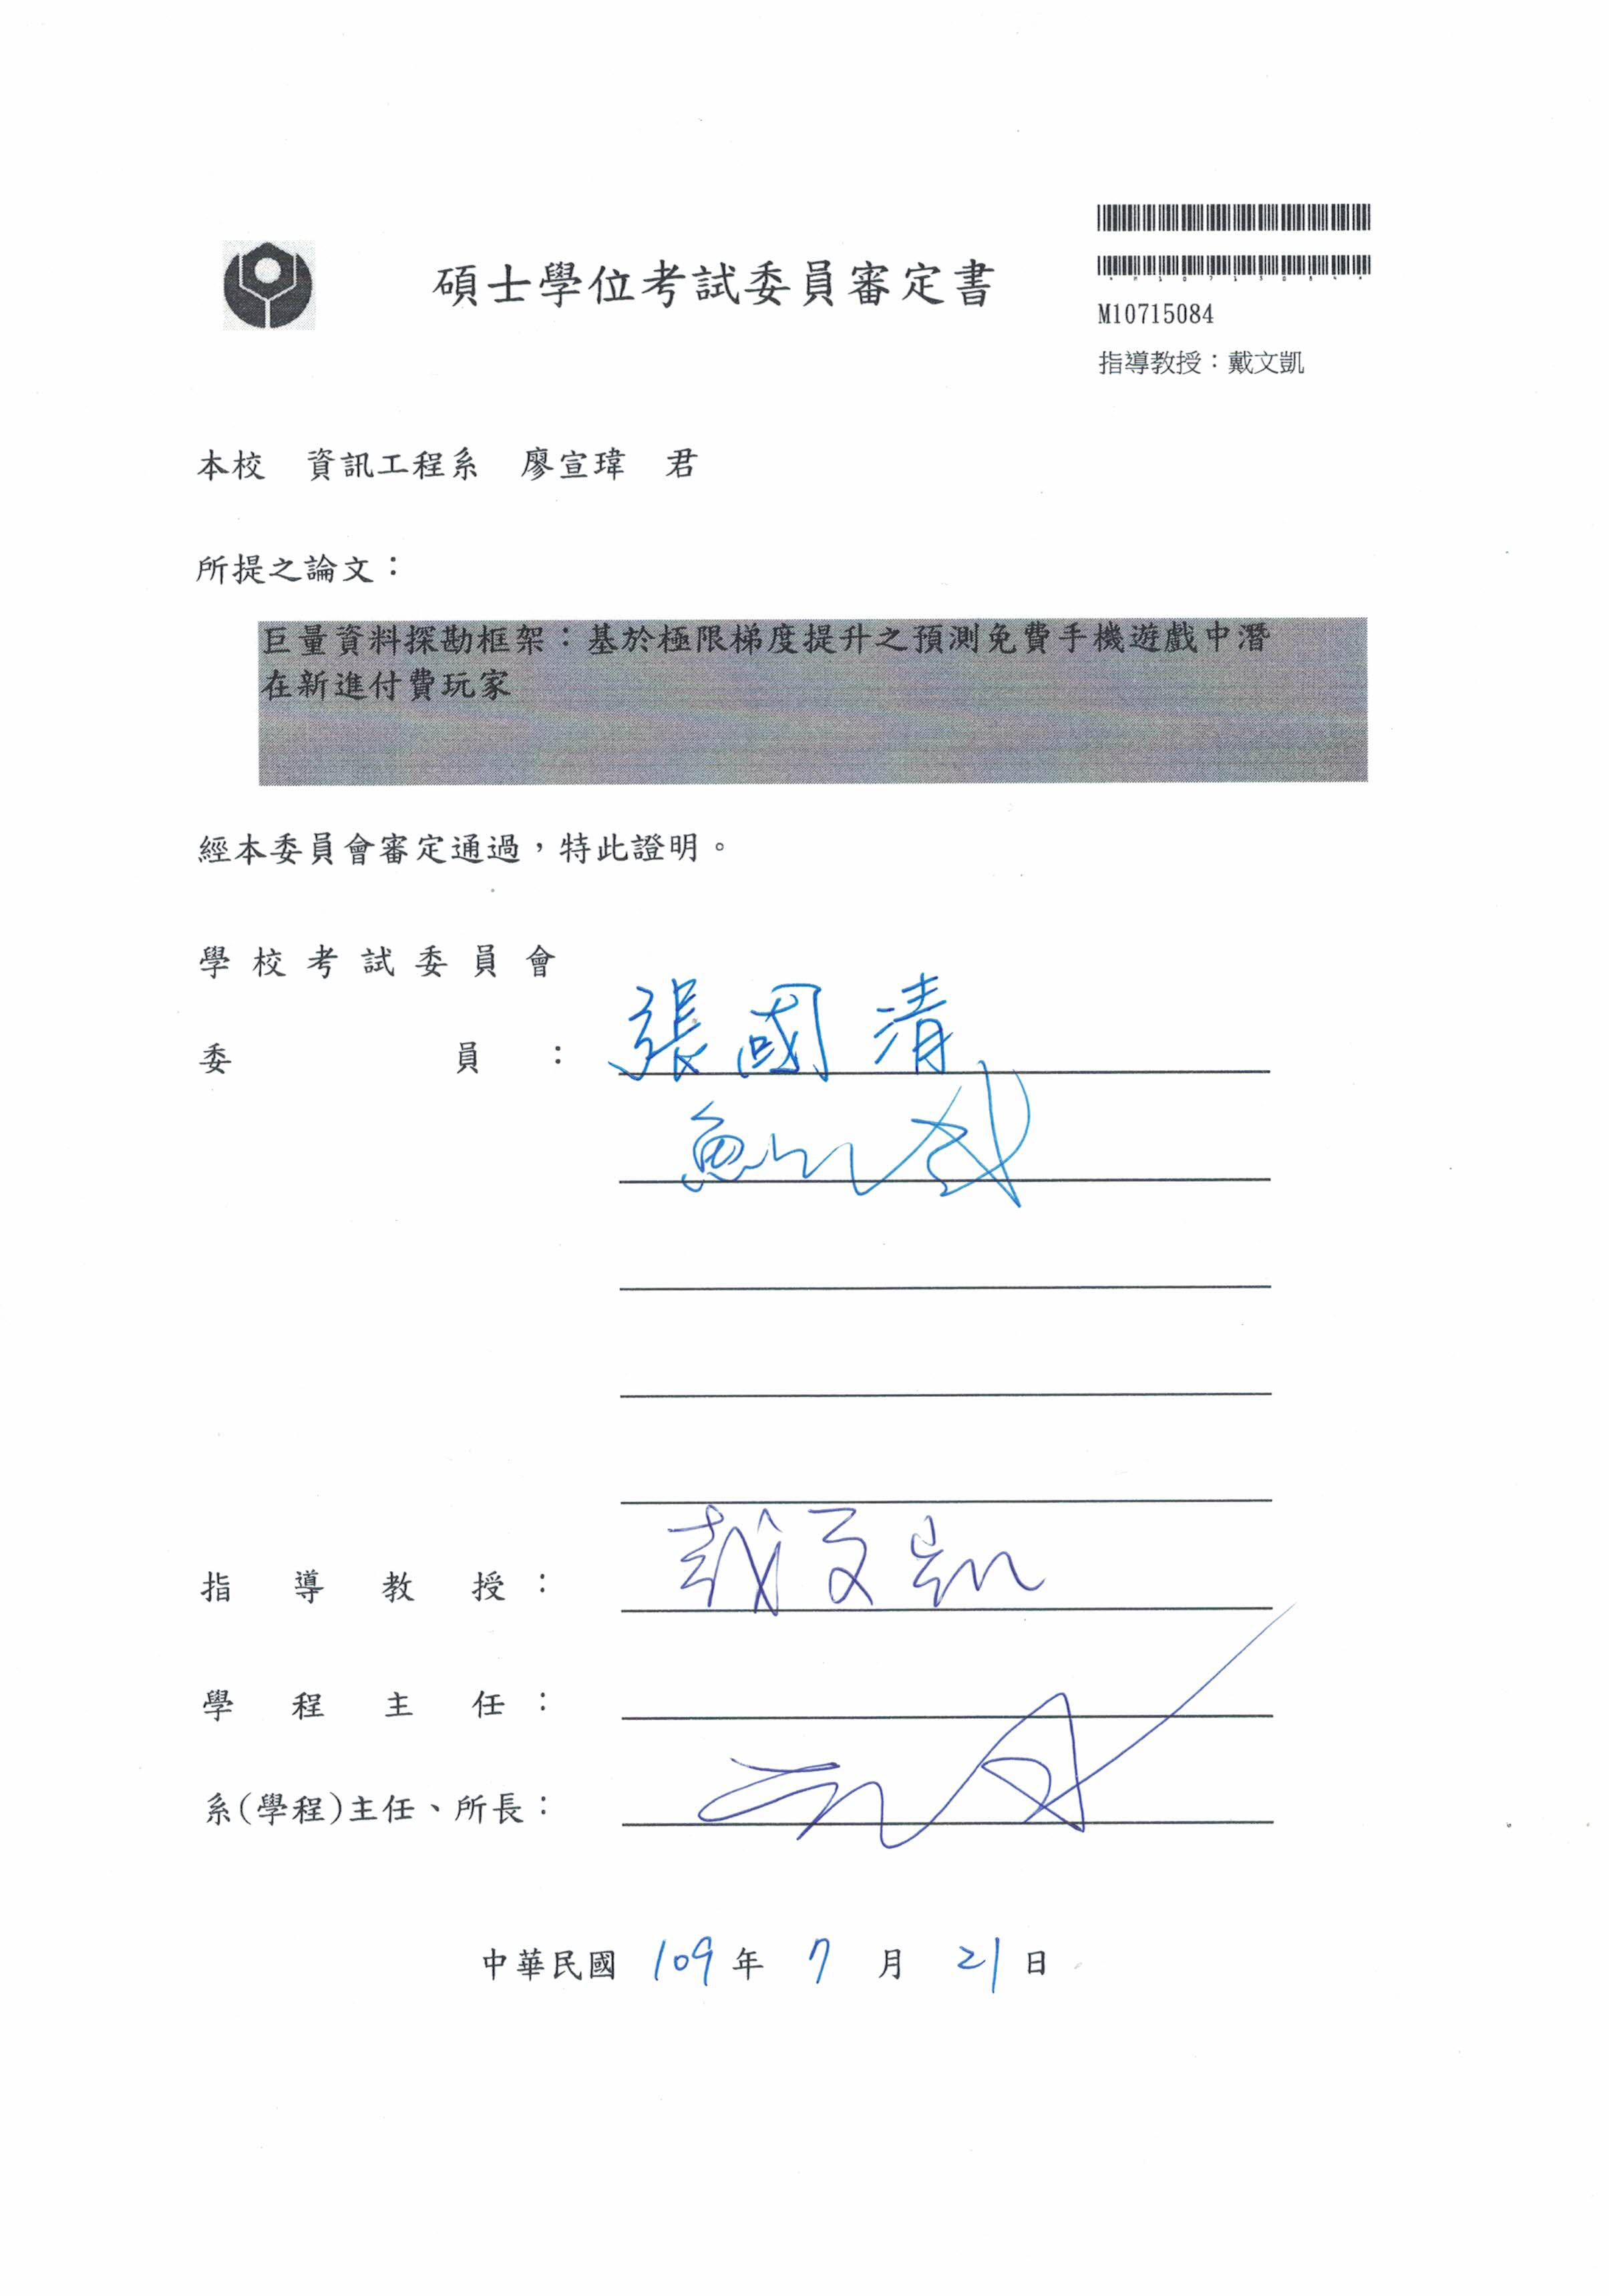
\includepdf[pages=-]{frontpages/reference_02.png} %審定書

% 判斷是否要浮水印?
\ifx\mywatermark\undefined 
  \thispagestyle{empty}  % 無頁碼、無 header (無浮水印)
\else
  \thispagestyle{EmptyWaterMarkPage} % 無頁碼、有浮水印
\fi

%%%%%%%%%%%%%%%%%%%%%%%%%%%%%%%%%%%%%%%%%%%%%%%%%%%%%%%%%%%%%%%
%%no page number
%% create an entry in table of contents for 書名頁
%\addcontentsline{toc}{chapter}{\nameInnerCover}
%
%
%% aligned to the center of the page
%\begin{center}
%% font size (relative to 12 pt):
%% \large (14pt) < \Large (18pt) < \LARGE (20pt) < \huge (24pt)< \Huge (24 pt)
%% Set the line spacing to single for the titles (to compress the lines)
%\renewcommand{\baselinestretch}{1}   %行距 1 倍
%% it needs a font size changing command to be effective
%%中文題目
%\Large{\cTitle}\\ %%%%%
%\vspace{1cm}
%% 英文題目
%\Large{\eTitle}\\ %%%%%
%%\vspace{1cm}
%\vfill
%% \makebox is a text box with specified width;
%% option s: stretch
%% use \makebox to make sure
%% 「研究生:」 與「指導教授:」occupy the same width
%\makebox[3cm][s]{\large{研 究 生:}}
%\makebox[3cm][l]{\large{\myCname}} %%%%%
%\hfill
%\makebox[2cm][s]{\large{Student: }}
%\makebox[5cm][l]{\large{\myEname}}\\ %%%%%
%%
%%\vspace{1cm}
%%
%\makebox[3cm][s]{\large{指導教授:}}
%\makebox[3cm][l]{\large{\advisorCnameA}} %%%%%
%\hfill
%\makebox[2cm][s]{\large{Advisor: }}
%\makebox[5cm][l]{\large{\advisorEnameA}}\\ %%%%%
%%
%% 判斷是否有共同指導的教授 B
%\ifx \advisorCnameB  \itsempty
%\relax % 沒有 B 教授,所以不佔版面,不印任何空白
%\else
%%共同指導的教授B
%\makebox[3cm][s]{}
%\makebox[3cm][l]{\large{\advisorCnameB}} %%%%%
%\hfill
%\makebox[2cm][s]{}
%\makebox[5cm][l]{\large{\advisorEnameB}}\\ %%%%%
%\fi
%%
%% 判斷是否有共同指導的教授 C
%\ifx \advisorCnameC  \itsempty
%\relax % 沒有 C 教授,所以不佔版面,不印任何空白
%\else
%%共同指導的教授C
%\makebox[3cm][s]{}
%\makebox[3cm][l]{\large{\advisorCnameC}} %%%%%
%\hfill
%\makebox[2cm][s]{}
%\makebox[5cm][l]{\large{\advisorEnameC}}\\ %%%%%
%\fi
%%
%% Resume the line spacing to the desired setting
%\renewcommand{\baselinestretch}{\mybaselinestretch}   %恢復原設定
%\large %it needs a font size changing command to be effective
%%
%\vfill
%\makebox[4cm][s]{\large{\univCname}}\\% 校名
%\makebox[6cm][s]{\large{\deptCname}}\\% 系所名
%\makebox[3cm][s]{\large{\degreeCname 論文}}\\% 學位名
%%
%%\vspace{1cm}
%\vfill
%\large{A Thesis}\\%
%\large{Submitted to }%
%%
%\large{\fulldeptEname}\\%系所全名 (英文)
%%
%%
%\ifx \collEname  \itsempty
%\relax % 沒有學院名 (英文),所以不佔版面,不印任何空白
%\else
%% 有學院名 (英文)
%\large{\collEname}\\% 學院名 (英文)
%\fi
%%
%\large{\univEname}\\%校名 (英文)
%%
%\large{in Partial Fulfillment of the Requirements}\\
%%
%\large{for the Degree of}\\
%%
%\large{\degreeEname}\\%學位名(英文)
%
%\large{in}\\
%%
%\large{\deptEname}\\%系所短名(英文;表明學位領域)
%%
%\large{\eMonth\ \eYear}\\%月、年 (英文)
%%
%\large{\ePlace}% 學校所在地 (英文)
%\vfill
%\large{中華民國}%
%\large{\cYear}% %%%%%
%\large{年}%
%\large{\cMonth}% %%%%%
%\large{月}\\
%\end{center}
%% restore the font size to normal
%\normalsize
%\clearpage


%%%%%%%%%%%%%%%%%%%%%%%%%%%%%%%%%%%%%%%%%%%%%%%%%%%%%%%%%%%%%%%%%%%%%
%%%%%%%%%%%%%%%%%%%%%%%%%%%%%%%
%       論文口試委員審定書 (計頁碼,但不印頁碼) 
%%%%%%%%%%%%%%%%%%%%%%%%%%%%%%%
%
% insert the printed standard form when the thesis is ready to bind
% 在口試完成後,再將已簽名的審定書放入以便裝訂
% create an entry in table of contents for 審定書
% 目前送出空白頁

%\newpage{\thispagestyle{empty}\addcontentsline{toc}{chapter}{\nameCommitteeForm}\mbox{}\clearpage}%


%%%%%%%%%%%%%%%%%%%%%%%%%%%%%%%
%       中文摘要 
%%%%%%%%%%%%%%%%%%%%%%%%%%%%%%%
%
\newpage
\thispagestyle{plain}  % 無 header,但在浮水印模式下會有浮水印
% create an entry in table of contents for 中文摘要
\phantomsection
\addcontentsline{toc}{chapter}{\nameCabstract}

% aligned to the center of the page
\begin{center}
	\makebox[5cm][s]{\LARGE{中文摘要}}\\
\end{center}
% Resume the line spacing to the desired setting
\renewcommand{\baselinestretch}{\mybaselinestretch}
%it needs a font size changing command to be effective
% restore the font size to normal
\normalsize
%%%%%%%%%%%%%
\noindent
目前市面上之手機遊戲多以免費遊玩商業模式(Free-to-Play, F2P)為主,使得遊戲內購買( In-App Purchase, IAP)顯得越來越重要,已然成為遊戲開發商營運之重點,為了能夠推出成功吸引各式玩家的精準行銷,需要資料分析團隊針對付費玩家進行研究,並且希望能夠在新進玩家族群中,成功預測出潛在付費玩家,以利提升IAP的意願,因此,如何在付費玩家資料中,有效探勘出資料特徵並透過機器學習進行預測,則為此次研究的目標。

本論文對此議題提出一巨量資料探勘框架,將需先將資料進行前處理以及預測前之資料分析,隨後訓練機器學習與其最佳化處理,最後再依預測之結果導入資料特徵重要性分析之中,完成整體預測與分析之工作,此框架將由四大階段組成: (1) 資料前處理階段、(2) 資料分析階段、(3) 機器學習階段及(4) 預測結果分析階段。

根據實驗結果,藉由我們提出的巨量資料探勘框架,利用無價值玩家觀察期清理了無價值的資料,並藉由付費玩家定義期準備了付費玩家與非付費玩家目標值,利用資料特徵探勘期探勘出了有價值的玩家遊戲行為軌跡。透過探索性資料分析(Exploratory Data Analysis, EDA)找出不合理資料特徵與高資訊量資料特徵,推測出有價值的資料特徵。能夠經由學習模型之預測,預測出潛在之新進付費玩家,並依其預測結果,分析資料特徵重要性,了解到玩家消費原因與遊戲之連動性。整體來說,該框架將能使得預測付費玩家之時間成本與人力成本有效降低,並得到對於行銷有利的資訊。

關鍵字:付費預測、免費遊玩遊戲、巨量資料、資料探勘、機器學習、極限梯度提升
\newpage

%%%%%%%%%%%%%%%%%%%%%%%%%%%%%%%
%       英文摘要 
%%%%%%%%%%%%%%%%%%%%%%%%%%%%%%%
%
\thispagestyle{plain}  % 無 header,但在浮水印模式下會有浮水印
% create an entry in table of contents for 英文摘要
\phantomsection
\addcontentsline{toc}{chapter}{\nameEabstract}
% aligned to the center of the page
\begin{center}
	% \renewcommand{\baselinestretch}{1}   %行距 1 倍
	\makebox[\width][s]{\LARGE{ABSTRACT}}\\
\end{center}
% Resume the line spacing the desired setting
\renewcommand{\baselinestretch}{\mybaselinestretch}   %恢復原設定
%\large %it needs a font size changing command to be effective
% restore the font size to normal
\normalsize
%%%%%%%%%%%%%

In recent years, most mobile game developers focus on free-to-play (F2P) games. However, it is extremely difficult for F2P games to define whether players are churning, which makes game operators hard to retain players. In addition, new players have a higher churn rate. Therefore, if operators can accurately predict the new players that may churn, they can immediately adopt a retention strategy to lost players, looking forward that this will increase the retention rate of new players and thus effectively increase revenue.

This thesis proposes a machine learning framework for this topic, which is composed of five major stages: (1) pre-processing stage, (2) analysis stage, (3) machine learning stage, (4) feature extraction analysis stage and (5) businese application analysis stage. To be specific, the framework will need to process the data and data analysis before prediction, and train the model via machine learning algorithm, then analyze important features with the prediction results. Finally, by using surrogate model, the framework will be able to find out the patterns of player churn.

Keywords: New Player, Churn Prediction, Free-to-Play, Machine Learning

%%%%%%%%%%%%%%%%%%%%%%%%%%%%%%%
%       誌謝 
%%%%%%%%%%%%%%%%%%%%%%%%%%%%%%%
%
% Acknowledgment
\newpage
% \chapter*{\protect\makebox[5cm][s]{\nameAckn}} %\makebox{} is fragile; need protect
\phantomsection
\addcontentsline{toc}{chapter}{\nameAckn}
\begin{center}
	\makebox[5cm][s]{\LARGE{誌謝}}\\
\end{center}

非常感謝指導教授戴文凱博士,在我的碩士生涯中給予我許多的指導,在討論研究時,老師都會適時地指出不足之處;在撰寫論文時,老師也都會幫忙審查,並時常會叮嚀我注意小細節,讓我能順利的完成本論文,再次感謝老師的教導與協助。

另外,特別感謝張國清博士,時常在我研究時給予我建議,並指正我錯誤的部分,讓我的實驗結果有不錯的表現;在我於公司實習時,也都會額外花時間教學與照顧,讓我額外學到許多與產業應用相關的部份,再次感謝張博士的鼎力相助。

最後感謝一路上陪伴我求學的家人們,在我感到壓力時,能給我許多溫暖與依靠;在我遇到困難時,能給我極大的鼓勵與支持,讓我能夠持續堅持下去,且不顧一切地繼續往前走,真的很感謝我的家人們。

%%%%%%%%%%%%%%%%%%%%%%%%%%%%%%%
%       目錄 
%%%%%%%%%%%%%%%%%%%%%%%%%%%%%%%
%
% Table of contents
\newpage
\renewcommand{\contentsname}{\protect\makebox[5cm][s]{\nameToc}}
%\makebox{} is fragile; need protect
\phantomsection
\addcontentsline{toc}{chapter}{\nameToc}
\tableofcontents

%%%%%%%%%%%%%%%%%%%%%%%%%%%%%%%
%       圖目錄 
%%%%%%%%%%%%%%%%%%%%%%%%%%%%%%%
%
% List of Figures
\newcommand{\loflabel}{圖}
\newpage
\renewcommand{\numberline}[1]{\loflabel~#1\hspace*{1em}}
\renewcommand{\listfigurename}{\protect\makebox[5cm][s]{\nameTof}}
%\makebox{} is fragile; need protect
\phantomsection
\addcontentsline{toc}{chapter}{\nameTof}
\listoffigures

%%%%%%%%%%%%%%%%%%%%%%%%%%%%%%%
%       表目錄 
%%%%%%%%%%%%%%%%%%%%%%%%%%%%%%%
%
% List of Tables
\newcommand{\lotlabel}{表}
\newpage
\renewcommand{\numberline}[1]{\lotlabel~#1\hspace*{1em}}
\renewcommand{\listtablename}{\protect\makebox[5cm][s]{\nameLot}}
%\makebox{} is fragile; need protect
\phantomsection
\addcontentsline{toc}{chapter}{\nameLot}
\listoftables

%%%%%%%%%%%%%%%%%%%%%%%%%%%%%%%
%       演算法目錄 
%%%%%%%%%%%%%%%%%%%%%%%%%%%%%%%
%
% List of Figures
%\newpage
%\renewcommand{\listalgorithmname}{\protect\makebox[5cm][s]{\nameToa}}
%\makebox{} is fragile; need protect
%\addcontentsline{toc}{chapter}{\nameToa}
%\listofalgorithms


%%%%%%%%%%%%%%%%%%%%%%%%%%%%%%%
%       符號說明 
%%%%%%%%%%%%%%%%%%%%%%%%%%%%%%%
%
% Symbol list
% define new environment, based on standard description environment
% adapted from p.60~64, <<The LaTeX Companion>>, 1994, ISBN 0-201-54199-8
\newcommand{\SymEntryLabel}[1]%
{\makebox[3cm][l]{#1}}

\newenvironment{SymEntry}
  {\begin{list}{}%
      {\renewcommand{\makelabel}{\SymEntryLabel}%
       \setlength{\labelwidth}{3cm}%
       \setlength{\leftmargin}{\labelwidth}%
      }%
  }%
  {\end{list}}
%
\newpage
\phantomsection
\chapter*{\protect\makebox[5cm][s]{\nameSlist}} %\makebox{} is fragile; need protect
\addcontentsline{toc}{chapter}{\nameSlist}
%
% this file is encoded in utf-8
% v1.7
% 各符號以 \item[] 包住,然後接著寫說明
% 如果符號是數學符號,應以數學模式表示,以取得正確的字體
% 如果符號本身帶有方括號,則此符號可以用大括號 {} 包住保護
\begin{SymEntry}

    \item[$O$]
    觀察期天數

    \item[$R$]
    挽留期天數
    
    \item[$P$]
    表現期天數
    
    \item[$class\ 1$]
    付費玩家

    \item[$class\ 0$]
    非付費玩家

    \item[$X$]
    訓練資料集占比
    
    \item[$Y$]
    測試資料集占比
    
    \item[$N_1$]
    流失玩家樣本數

    \item[$N_0$]
    非流失玩家樣本數
    
    \item[$G(\ )$]
    $Gini\ Impurity$

    \item[$GI(\ )$]
    $Gini\ Importance$

    \item[$fi(\ )$]
    資料特徵重要性 ( $Feature\ Importance$ )

    \item[$D$]
    某節點

    \item[$D_p$]
    父節點

    \item[$D_{left}$]
    左子節點

    \item[$D_{right}$]
    右子節點

    \item[$N_p$]
    父節點樣本數

    \item[$N_{left}$]
    左子節點樣本數

    \item[$N_{right}$]
    右子節點樣本數

    \item[$x$]
    欲求其重要性之資料特徵

    \item[$k$]
    節點分割時所用資料特徵為$x$之所有節點

    \item[$l$]
    樹中所有節點

    \item[$t$]
    學習模型中的所有樹

\end{SymEntry}


\newpage
\setcounter{page}{1}
\pagenumbering{arabic}
%% 論文本體頁碼回復為阿拉伯數字計頁,並從頭起算
%\pagenumbering{arabic}
%%%%%%%%%%%%%%%%%%%%%%%%%%%%%%%%

	%----------------------------------------------------------------------------------------------------------------------------------------------------------
	% main body 論文主體。建議以「章」為檔案分割的依據。
	% 以下為建議的命名分類
	%   introduction.tex   related_work.tex  protocol.tex  evaluation.tex  conclusion.tex
	% 做為這幾個「章」的檔案名稱,並將檔案存放於資料夾 sections/ 下
	% 實際命名方式可以隨你意
	% 在撰寫各章草稿時,可以把其他章節關掉 (行首加百分號)
	
	\chapter{緒論}

\section{研究背景與動機}

對於許多遊戲商而言,準確預測玩家流失對於長期成功至關重要。近年來,手機遊戲商大多以免費遊戲為主,不再是以往的買斷制或月費制。在免費遊戲的模式之下,遊戲商之營收有非常顯著的成長,例如:「絕地要塞 2」 ( Team Fortress 2 ) 原本為買斷制型式遊戲,新收入的來源僅限於沒購買過遊戲的人,這樣的商業模式與他們的發展策略並不完全吻合。於是,在 2011 年改為免費遊戲,除了擴大玩家受眾,還透過遊戲不斷地更新保持玩家的興趣。最終,遊戲營收提高達 12 倍之多~\cite{miller2012gdc}。但是,免費遊戲在定義是否為流失玩家上極為困難,一旦玩家想離開了隨時都能停止遊玩,沒有必要告訴遊戲商其決定,遊戲商也容易因此失去挽回玩家的機會。

根據哈佛商業評論~\cite{HarvardBusiness}中指出,企業爭取一個新顧客的成本是保留老顧客成本的 5 倍。一個公司如果能將其顧客流失率降低 5\%,其利潤就能增加 25\% - 85\%。也就是說,獲得一個新玩家的成本比留住一個玩家要昂貴許多。因此,留住玩家成為重要議題,精準地預測玩家流失,即使是微小地提升,也可能導致營收有顯著的提升。

另外,根據網站 Swrve~\cite{SwrveNewPlayerReport} 於 2014 年提供的報告指出,數十款的遊戲中,有 19.3\% 的新玩家只玩一次特定遊戲,新玩家的次日留存率為 33.9\%,而第 30 天的留存率只剩下 5.5\%。而 Mustač 等人~\cite{SupervisedMachineLearning}則是針對歐洲一款休閒遊戲進行研究,研究中可以看到,此遊戲有大約 60\% 的玩家在玩了一天後就離開了,3 天後,玩家們只剩下大約 20\% 。上述的 2 份報告都清楚表明了新進玩家的流失率是很嚴重的問題。因此,本文將針對新進玩家做流失預測分析,希望能因此提高新進玩家的留存率,進而有效地增加營收。

\section{研究目標}

本論文的研究目標是預測免費遊戲的新進玩家是否會流失。透過新進玩家在遊戲初期的遊玩歷程和儲值紀錄等特徵訓練出準確率最高的模型,並藉由模型的結果分析各個特徵的突出性,來進行玩家流失原因的解釋說明,甚至能從中了解玩家們的喜好、趨勢,也可以讓市場操作人員有挽留玩家的操作依據,有了明確的挽留策略就能夠對症下藥,藉此來強化留存,並進一步增加營收。

\section{研究方法概述}

本論文將新進玩家創帳號後的天數切分為三個時期:(1) 觀察期:玩家創帳號後前幾天,會將此時期的玩家行為軌跡作為資料特徵來訓練模型; (2) 挽留期:於觀察期之後,作為給市場操作人員實施挽留策略的時間; (3) 表現期:於挽留期之後,決定玩家是否流失,如果玩家在此時期有任一登入紀錄則視為非流失玩家,反之將視為流失玩家。

此外,本文提出一巨量資料探勘框架:此框架將由五大階段組成, (1) 資料前處理階段:首先從資料庫群中整合所有需要的資料,並過濾掉無價值玩家,再著手目標值準備並建立資料特徵,以利後續分析及機器學習使用; (2) 資料分析階段:使用前階段產出之資料,透過統計圖表來觀察資料特性,進行探索性資料分析 ( Exploratory Data Analysis )~\cite{tukey1977exploratory},藉由流失玩家與非流失玩家的資料分佈,來觀察資料特徵是否可以提供給學習模型較多之資訊; (3) 機器學習階段:首先將處理後的資料集分割為訓練集及測試集,隨後針對訓練集進行多數群樣本權重值縮小,並透過網格搜索 ( Grid Search )~\cite{wiki:HyperparameterOptimization}與交叉驗證 ( Cross Validation )~\cite{wiki:CrossValidation}找出機器學習模型的最佳超參數,以獲得最佳模型,其中學習模型選用決策樹 ( Decision Tree )~\cite{breiman1984classification}、隨機森林 ( Random Forest )~\cite{breiman2001random}及極限梯度提升 ( Extreme Gradient Boosting )~\cite{chen2016xgboost},最後藉由測試集來驗證評估最佳模型,產出預測結果; (4) 預測結果分析階段:使用前階段產出之預測結果進行資料特徵重要性分析,透過計算各資料特徵於各學習模型中之基尼重要性 ( Gini Importance )~\cite{GiniImportance},以利更加了解及解釋資料特徵與遊戲所提供之體驗綜合評估;(5) 產業應用分析階段:參考代理人模型 ( Surrogate Model )~\cite{wiki:SurrogateModel},用較簡單的模型來模擬較複雜的模型,能協助了解流失玩家的行為規則,作為市場操作人員的操作依據。

在方法驗證上,本論文將藉由混淆矩陣 ( Confusion Matrix ) 所延伸之 ROC Curve ( Receiver Operating Characteristic Curve )~\cite{fawcett2006introduction}與 PR Curve ( Precision-Recall Curve )~\cite{article}來協助驗證學習模型之優劣,並同時利用 Weighted F$_{\beta}$ - Score~\cite{Goutte2005API}來選出最佳模型與最佳參數解,隨後計算特徵重要性 ( Feature Importance ) 於各資料特徵中,以了解到何者於學習模型中貢獻了最多的資訊量,以利學習模型進行訓練與分類。

\section{研究貢獻}

本論文之研究貢獻為:

\begin{enumerate}
    \item 訓練一新進玩家流失預測模型並運用於遊戲領域,利用其預測結果從中了解玩家流失的原因與動機,並作為市場操作人員後續挽留玩家的操作依據,以強化留存並進一步增加營收。
    \item 提出一建立資料特徵的方法:對資料集以統計手法建立資料特徵,並用多個時間框架做拆分,以獲得第一層特徵變數,再對第一層特徵變數做計算,進一步來得到第二層特徵變數,如變化量特徵等。
    \item 於資料集中進行資料特徵之探勘,藉由不同種類與面向之方式,挑選出適合用來呈現流失玩家的資料。
    \item 整理出適合於不平衡資料集中的評估值方式,將對於學習模型之預測結果提供合理的評估,進而進行比較。
    \item 整理出資料特徵重要性之計算,以利分析資料特徵的突出性與其貢獻的資訊量。
    \item 透過代理人模型了解流失玩家的行為規則,能做為市場操作人員的操作依據,方便產業應用。
\end{enumerate}

\section{本論文之章節結構}

本論文第~\ref{cha:RelatedWork}~章為文獻探討,探討關於資料前處理、學習模型選擇、資料不平衡處理以及其評估方式的相關文獻。第~\ref{cha:Method}~章為研究方法,詳述講述各階段之研究流程,並分為五節來介紹資料前處理、資料分析、機器學習、預測結果分析及產業應用分析。第~\ref{cha:Evaluation}~章為實驗結果與分析,分為六節:第~\ref{sec:SystemStructure}~節實驗系統架構;第~\ref{sec:DataPreprocessEvaluation}~節資料前處理評估;第~\ref{sec:DataAnalysisEvaluation}~節資料分析評估;第~\ref{sec:MachineLearningEvaluation}~節機器學習評估;第~\ref{sec:PredictionResultAnalysisEvaluation}~節預測結果分析評估;第~\ref{sec:ApplicationAnalysisEvaluation}~節產業應用分析評估。第~\ref{cha:Conclusions}~章為結論與未來研究,總結本論文提出的方法與實驗結果,並討論未來的研究方向。
\newpage
%%% 	\chapter{文獻探討}
\label{cha:RelatedWork}

本章節針對免費遊戲興起介紹,並探討關於資料前處理、學習模型選擇、資料不平衡處理以及其評估方式的相關文獻。

\section{免費遊戲興起}

免費遊戲,是一種玩家無需支付任何費用,即可遊玩該遊戲之大部分內容,與付費型遊戲(買斷制或月費制)形成對比。在免費遊戲中,遊戲商可以藉由遊戲內購買或遊戲內置入廣告等方式來賺取營收~\cite{wiki:f2p}。近幾年內,遊戲商皆轉以開發免費遊戲為主,因其類型所帶來之營收,已遠大於付費型遊戲~\cite{lee2018game}。另外,免費遊戲還能夠有效的讓玩家流失量降低,透過其無需支付任何費用就能遊玩遊戲的特性,使玩家進入遊戲的門檻大為降低~\cite{10.1007/978-3-030-27355-2_10}。

雖然免費遊戲能讓玩家流失量降低,但相對的,對於玩家是否流失變得極難定義,因為玩家可以在沒有任何通知的情況下停止遊戲,沒有明確的流失事件,例如玩家取消訂閱。儘管玩家流失模型在商業領域已經存在了幾十年,但隨著機器學習方法近年來的進步,它們的複雜性和準確性也都在提升,因此,即使在高維數據上,也可以應用極限梯度提升等機器學習來創建非常準確的模型~\cite{XGBoostTemporalData}。

\section{資料前處理}

在將巨量資料應用於機器學習前,資料的前處理也是極為重要,相較於在學習模型上進行深入研究與改進,透過資料特徵之轉化及選擇顯得更為重要且有效~\cite{SupervisedMachineLearning}~\cite{lee2018game}~\cite{XGBoostTemporalData}。

首先將對資料進行清理,只收集有價值之資料,例如:Tamassia等人只收集遊玩時間超過給定門檻之玩家~\cite{tamassia2016predicting}、Periáñez等人只收集消費金額遠高於一般玩家者~\cite{perianez2016churn}或Runge等人只取付費玩家中前10 \%者~\cite{runge2014churn},上述之清理方式皆只著重於具有高資訊量的資料,而不將無價值的資料放入機器學習中。

而針對資料特徵之探勘,Sifa 等人~\cite{sifa2015predicting}將探勘玩家基本資料及玩家行為,再將其進行轉化,例如:取平均值與偏差值於玩家遊玩時間、將玩家國籍分類等。Xie等人~\cite{PredictionWithEventFrequency}使用遊戲內的事件發生頻率來預測玩家對遊戲的參與度。Lee等人~\cite{lee2016predicting}將探勘玩家行為、玩家購買商品數量、玩家遊戲內交易及玩家遊戲內社交,主要針對玩家每日於遊戲內的行為軌跡。Gregory~\cite{XGBoostTemporalData}透過相對時間及絕對時間建立新的特徵,以提升資料集的特徵數量。Hadiji等人~\cite{6932876}將探勘玩家消費商品數量、玩家遊玩天數等。

\section{學習模型選擇}

在機器學習中,於分類預測的應用上,樹狀結構之學習模型最為主流且有效,因其建樹之方式,可以清楚的解釋該筆樣本之預測路徑,進而針對各資料特徵進行重要性的計算與分析~\cite{lee2018game}。另外,在樹狀結構之學習模型中,主流以裝袋算法 ( Bagging ) 及提升方法 ( Boosting ) 兩種建樹想法為準:

\begin{itemize}
    \item 裝袋算法:從訓練資料集中,隨機取樣並訓練成多份分類器,而每次訓練時會將資料取出後放回,並再次抽取,最後的預測結果將由多個分類器投票選出,採多數決,且各分類器間的權重關係皆為相等~\cite{breiman1996bagging},如圖~\ref{fig:Bagging}。例如:隨機森林~\cite{breiman2001random}即為裝袋算法 + 決策樹~\cite{breiman1984classification}。
    \item 提升方法:從訓練資料集中,每次訓練使用相同資料,而第 n 個分類器於訓練時,將針對第 n-1 個分類器分類錯誤的資料增大其權重值,以修正分錯的資訊,希望將分錯的資料減少,預測結果將由多個分類器投票選出,各分類器間的權重關係不同,錯誤率越低的分類器,擁有越高的權重~\cite{freund1999short},如圖~\ref{fig:Boosting}。例如:極限梯度提升~\cite{chen2016xgboost}即為提升方法 + 決策樹。
\end{itemize}

\begin{figure}[!htb]
    \begin{center}
      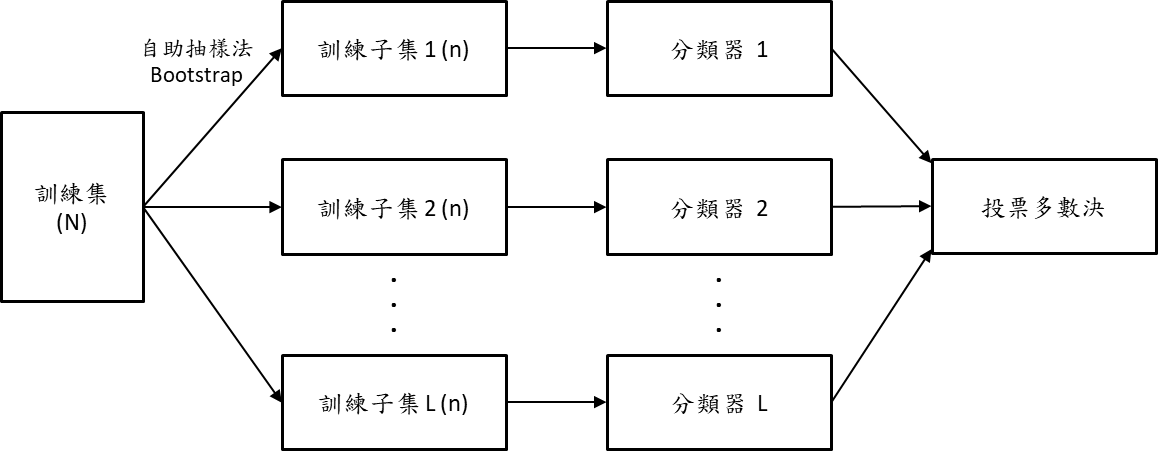
\includegraphics[width=1\textwidth]{figures/Image_Bagging.png}
      \caption[裝袋算法方式建樹示意圖]{裝袋算法方式建樹示意圖}
      \label{fig:Bagging}
    \end{center}
\end{figure}

\begin{figure}[!htb]
    \begin{center}
      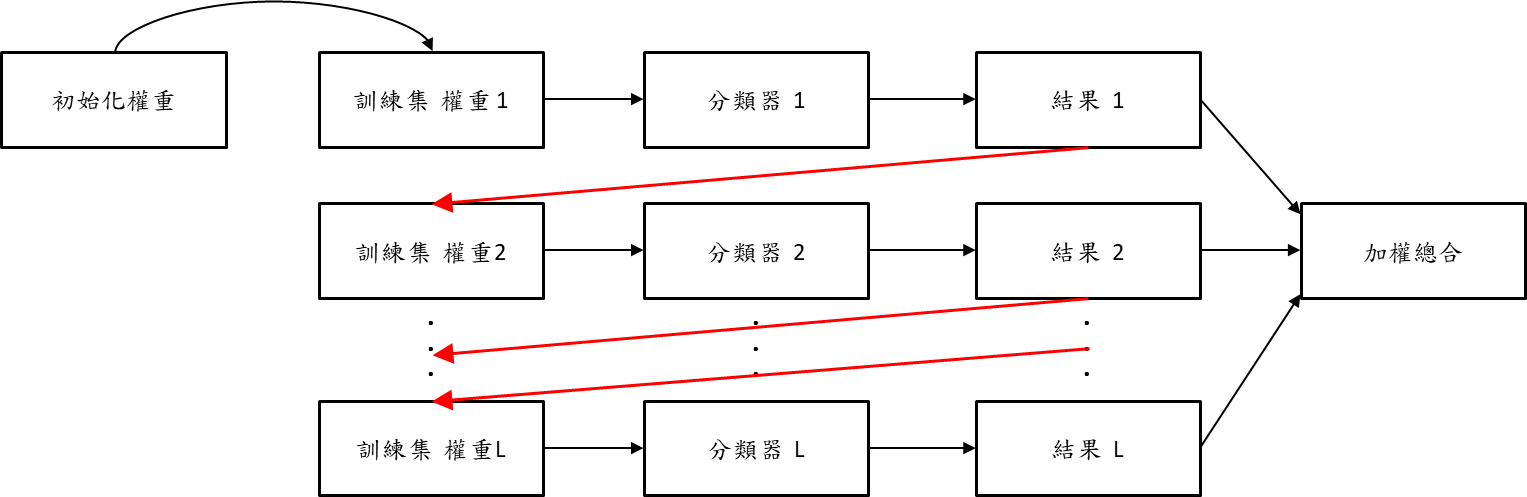
\includegraphics[width=1\textwidth]{figures/Image_Boosting.png}
      \caption[提升方法方式建樹示意圖]{提升方法方式建樹示意圖}
      \label{fig:Boosting}
    \end{center}
\end{figure}

Chen與Guestrin~\cite{chen2016xgboost}實作出高效率的梯度提升 ( Gradient Boosting ),稱其為極限梯度提升,除了使用提升方法建樹外,還針對錯誤修正的步驟,引入梯度下降法 ( Gradient Descent ) 的概念,加速了學習模型的收斂速度,使其修正錯誤的能力更加精準,大幅減少訓練的時間成本。近年來透過極限梯度提升來訓練的研究越來越多,且其預測能力皆有不錯的表現~\cite{XGBoostTemporalData}~\cite{martinez2020machine}~\cite{semenov2016performance}~\cite{janusz2017helping},明顯優於裝袋算法建樹方式的其他學習模型。
\newpage

從上述得知,選用樹狀結構之學習模型將有助於預測分類問題,且其中使用極限梯度提升之成效最佳。因此,為求本論文之預測新進玩家流失能夠達到預期,將採用決策樹、隨機森林與極限梯度提升來驗證樹狀結構之優勢以及極限梯度提升之最佳表現。

\section{資料不平衡處理及其評估方式}

在遊戲領域進行機器學習訓練時,往往會遭受到資料不平衡的影響;例如:於預測是否付費上,非付費玩家會遠多於付費玩家,導致付費玩家資料過少~\cite{sifa2015predicting}。於預測是否流失上,流失玩家會遠多於非流失玩家,導致非流失玩家資料過少~\cite{lee2016predicting},前述研究都採以針對資料集進行處理的方式解決資料不平衡,例如:SMOTE (Synthetic Minority Over-sampling Technique),於少數群添加模擬資料,使得少數群之樣本數與多數群相等~\cite{chawla2002smote}。而本論文不只預測玩家是否會流失,還需分析其原因,如在資料集中填入模擬資料,將會使得分析失準,無法得到有效的資訊,所以我們將採用在機器學習訓練時,放大少數群之樣本權重值,使得學習模型更加著重於少數群的資訊,如同提升方法建樹時,藉由權重值的不同,修正分類錯誤的資訊~\cite{freund1999short}。

在評估資料不平衡資料集時,如果單純計算學習模型之 Precision、Recall 或 F - Score~\cite{chinchor1993muc},將導致多數群之評估結果壓過少數群之評估結果,使得最終評估失真,無法有效驗證學習模型之成效。因此,在評估不平衡資料時,Sifa等人額外運用幾何平均數 ( Geometric Mean )~\cite{kubat1997learning}來評估學習模型之成效~\cite{sifa2015predicting}。藉由上述的概念,本論文將採用 Weighted F$_{\beta}$ - Score 來評估不平衡資料,使得少數群之評估不被多數群所壓過,使用樣本間的數量權重差來計算多數群與少數群的 F$_{\beta}$ - Score,希望能夠合理的評估學習模型間的表現。
%%% 	\chapter{研究方法}
\label{cha:Method}

針對遊戲領域巨量資料進行新進玩家流失預測,先將資料進行前處理以及預測前之資料分析,隨後訓練機器學習與其最佳化處理,最後再依預測之結果導入資料特徵重要性分析之中,完成整體預測與分析之工作。

為求研究效率能夠快速且有效,本論文對此議題運用一巨量資料探勘框架,圖~\ref{fig:Image_Framework} 為巨量資料探勘框架示意圖,此框架將由五大階段組成:

\begin{itemize}
  \item[■] 資料前處理階段:首先將從資料庫群中整合所有所需資料,並過濾出有價值之原始資料,再著手目標值準備、資料特徵探勘與特徵工程,以利後續分析及機器學習使用。
  \item[■] 資料分析階段:使用前階段產出之有價值原始資料進行探索性資料分析,透過統計圖表來觀察資料特性,藉由流失玩家與非流失玩家的資料分佈,來觀察資料特徵是否可以提供給學習模型較多之資訊。
  \item[■] 機器學習階段:首先將有價值原始資料集進行分割為訓練及測試集,隨後針對訓練集進行交叉驗證搭配配參數表,以獲得模型的最佳參數解,最後藉由測試集來驗證評估最佳模型,產出預測結果。
  \item[■] 預測結果分析階段:使用前階段產出之預測結果進行資料特徵重要性分析,以利更加了解及解釋資料特徵與遊戲所提供之體驗綜合評估。
  \item[■] 產業應用分析階段:參考代理人模型,用較簡單的模型來模擬較複雜的模型,能協助了解流失玩家的行為規則,作為市場操作人員的操作依據。
\end{itemize} 

\begin{figure}[!htb]
  \begin{center}
    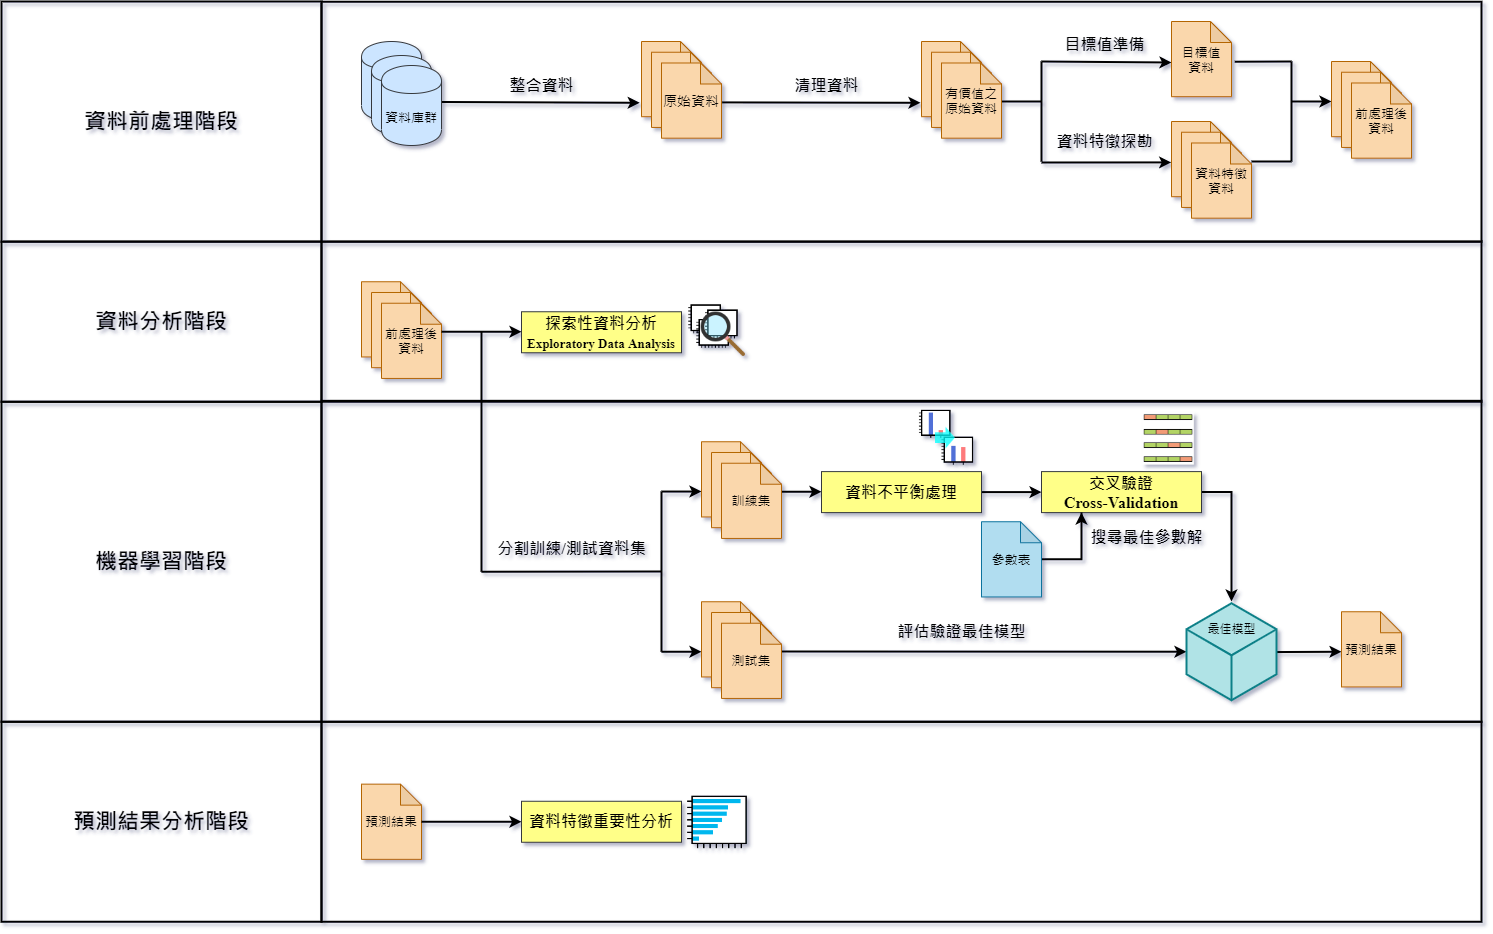
\includegraphics[width=1\textwidth]{figures/Image_Framework.png}
    \caption[本論文之巨量資料探勘框架示意圖]{本論文之巨量資料探勘框架示意圖}
    \label{fig:Image_Framework}
  \end{center}
\end{figure}
\newpage

\section{資料前處理階段}
\label{sec:DataPreProcess}

此階段將著重於資料之整合與過濾,為求能收集到有價值之原始資料,以提高後續分析研究之價值,同時進行目標值的準備、資料特徵的探勘與資料特徵工程,協助機器學習之訓練,目標產出有價值之玩家遊戲行為軌跡資料集。

\subsection{整合資料}
\label{subsec:DataIntegration}

首先資料庫群中之資料皆以天為單位,記錄了各項遊戲之玩家行為軌跡,如圖~\ref{fig:Image_Databases}。此步驟將依各項遊戲為整合目標,重整為多個原始資料集,每個原始資料集中,只會記錄該類遊戲之每位玩家行為軌跡,如圖~\ref{fig:Image_Integration},將可提升後續目標值準備及資料特徵探勘速度。

\begin{figure}[!htb]
  \begin{center}
    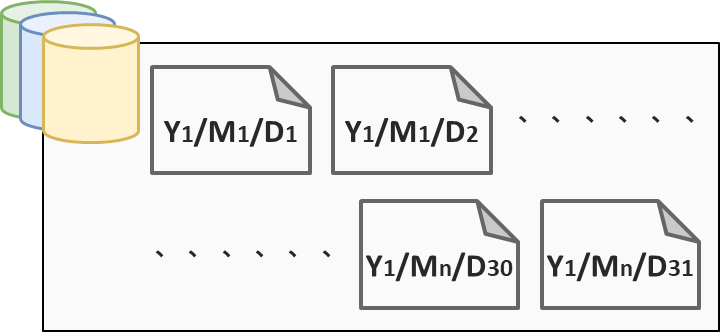
\includegraphics[width=0.6\textwidth]{figures/Image_Databases.png}
    \caption[資料庫群內資料之示意圖]{資料庫群內資料之示意圖}
    \label{fig:Image_Databases}
  \end{center}
\end{figure}

\begin{figure}[!htb]
  \begin{center}
    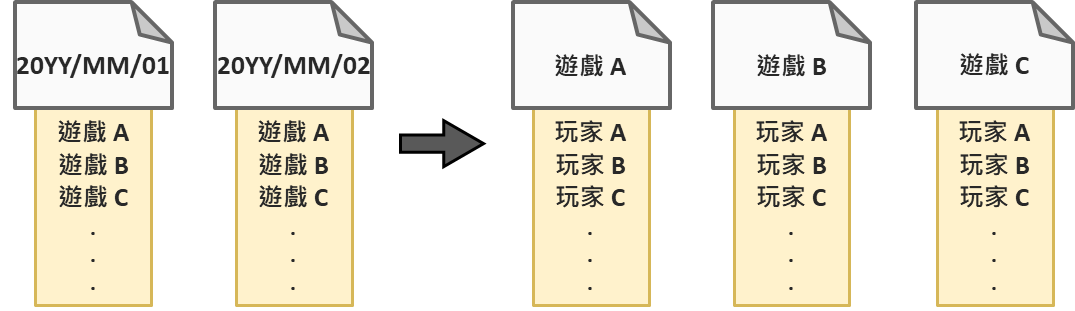
\includegraphics[width=0.85\textwidth]{figures/Image_Integration.png}
    \caption[依各項遊戲為整合目標之示意圖]{依各項遊戲為整合目標之示意圖}
    \label{fig:Image_Integration}
  \end{center}
\end{figure}

除了上述之玩家遊戲行為軌跡原始資料集外,還另外收集了玩家輪廓資料 ( 含國家、玩家等級等 ) 與玩家平台操作紀錄 ( 含消費紀錄、客訴紀錄等 ),最終此步驟將產出三大類原始資料集,如圖~\ref{fig:Image_OriginalDatasets}:

\begin{itemize}
  \item[■] 玩家輪廓資料 ( 含國家、玩家等級等 )
  \item[■] 玩家平台操作紀錄 ( 含消費紀錄、客訴紀錄等 )
  \item[■] 玩家遊戲行為軌跡
\end{itemize} 

\begin{figure}[!htb]
  \begin{center}
    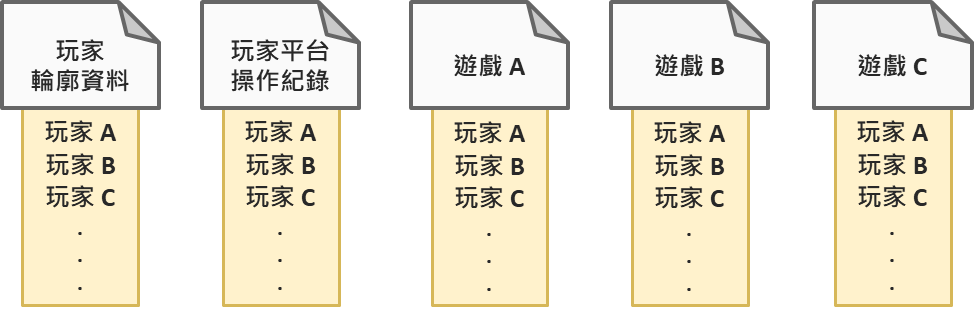
\includegraphics[width=0.75\textwidth]{figures/Image_OriginalDatasets.png}
    \caption[原始資料集示意圖]{原始資料集示意圖}
    \label{fig:Image_OriginalDatasets}
  \end{center}
\end{figure}
\newpage

\subsection{資料過濾}
\label{subsec:DataFilter}

此步驟將針對兩大議題:刪除空缺值與無價值玩家資料處理。

為了要在資料分析及訓練機器學習時,能夠更加準確的了解及預測真實遊戲玩家之特性與是否流失,需要透過上述之處理,來過濾掉潛在的無用資料,使得整體研究能夠聚焦於更有價值的資料上。

\subsubsection{刪除空缺值}
\label{subsubsec:MissingValueHandle}

為了後續資料特徵重要性分析,希望能保持著資料間的真實性,將採用直接刪去具有空缺值樣本的方式,而不對資料集填入經過處理之假數值,每筆樣本只要在任意資料特徵中擁有一空缺值,即視為欲刪除之對象。

圖~\ref{fig:Image_MissingValueHandle} 為刪除空缺值之示意圖,從圖中可以看出樣本ID 1及2分別在特徵3及1擁有空缺值,將對兩者予以刪除,故最後只留下樣本ID 0及3之資料。

\begin{figure}[!htb]
  \begin{center}
    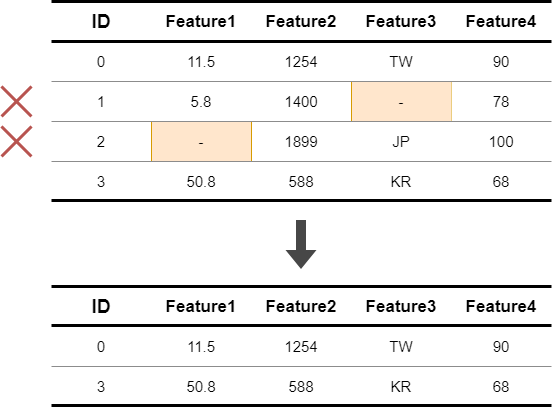
\includegraphics[width=0.7\textwidth]{figures/Image_MissingValueHandle.png}
    \caption[刪除空缺值示意圖]{刪除空缺值示意圖}
    \label{fig:Image_MissingValueHandle}
  \end{center}
\end{figure}

\subsubsection{無價值玩家資料處理}
\label{subsubsec:NonValuePlayerHandle}

對於遊戲領域巨量資料進行研究時,普遍會對所有玩家進行篩檢,以挑選出有價值之玩家族群,可使整體分析與預測更加貼近於真實遊戲情景。定義一時間框架於新進玩家創帳號後,又將其切分為三個時期:

\begin{itemize}
  \item [■] 觀察期:玩家創立帳號後前$O$天。觀察玩家在此時期的行為軌跡,並將對其進行特徵工程,因此,也將觀察期視為資料特徵探勘期。
  \item [■] 挽留期:觀察期之後前$R$天。作為市場操作人員實施挽留策略的時間。
  \item [■] 表現期:挽留期之後前$P$天。決定玩家是否流失,於玩家在觀察期有登入紀錄的前提下,如果玩家在此時期有任一登入紀錄則視為非流失玩家,反之將視為流失玩家。
\end{itemize}

如果該玩家創建帳號的日子較晚,尚未完整擁有上述三個時期的資料,將會造成後續特徵提取與目標值準備的不正確性,進而影響機器學習預測的準確度,因此將其視為無價值玩家,刪除該玩家及其所有行為軌跡。

圖~\ref{fig:Image_DataCleaning} 為判別有價值與無價值玩家之示意圖。從圖中可以看出,玩家1及玩家2已在創帳號後完整經歷觀察期、挽留期與表現期,故視為有價值玩家;而玩家3,因缺少完整的表現期資料,容易被誤判為流失玩家,故視為無價值玩家;玩家4,除了表現期的資料,觀察期資料也並不完整,若將其視為有價值玩家,其錯誤的資料特徵將會影響機器學習之訓練,故也視為無價值玩家。

\begin{figure}[!htb]
  \begin{center}
    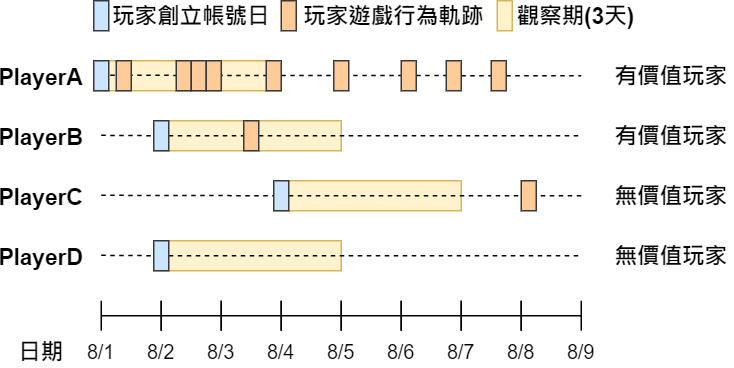
\includegraphics[width=0.8\textwidth]{figures/Image_DataCleaning.png}
    \caption[判別有價值與無價值玩家之示意圖]{判別有價值與無價值玩家之示意圖 (以$O$、$R$、$P$分別為 2、1、2 為例) }
    \label{fig:Image_DataCleaning}
  \end{center}
\end{figure}

經過前兩小節 \ref{subsubsec:MissingValueHandle} 及 \ref{subsubsec:NonValuePlayerHandle} 之處理後,最終此步驟將產出有價值之原始資料集,提供給後續分析及訓練機器學習使用。

\subsection{目標值準備}
\label{subsec:ClassPreparation}

此步驟將準備供機器學習使用之目標值,即為後續預測所需之$class$。定義目標值「非流失玩家」與「流失玩家」,分別代表$class\ 0$及$class\ 1$:

\begin{itemize}
  \item [■] 非流失玩家 ( $class\ 0$ ) :觀察期有登入紀錄的玩家中,表現期間有登入紀錄者,視為非流失玩家。
  \item [■] 流失玩家 ( $class\ 1$ ) :觀察期有登入紀錄的玩家扣除非流失玩家,剩餘者皆為流失玩家;表現期後才有登入紀錄者同樣視為流失玩家。
\end{itemize}

圖~\ref{fig:Image_ClassPreparation} 為定義非流失玩家與流失玩家之示意圖。從圖中可以看出玩家1及玩家2於觀察期及表現期中皆有登入紀錄,故定義為非流失玩家 ( $class\ 0$ ) ;而玩家3及玩家4則在表現期中無登入紀錄,故定義為流失玩家 ( $class\ 1$ ) ,即使玩家4在表現期後有登入紀錄,依舊將其視為流失玩家 ( $class\ 1$ ) 。

\begin{figure}[!htb]
  \begin{center}
    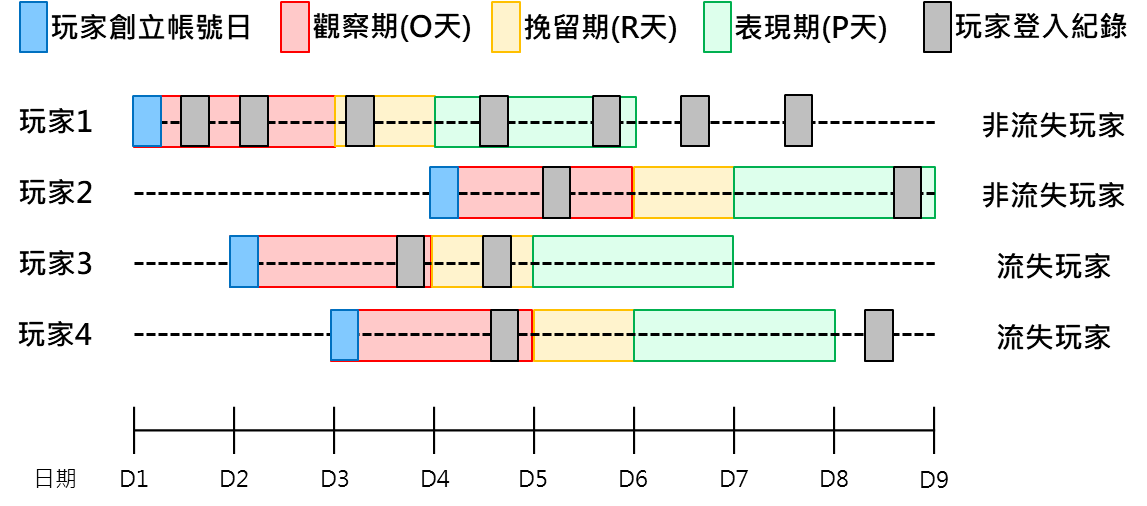
\includegraphics[width=0.8\textwidth]{figures/Image_ClassPreparation.png}
    \caption[非流失玩家與流失玩家之示意圖]{非流失玩家與流失玩家之示意圖 (以$O$、$R$、$P$分別為 2、1、2 為例) }
    \label{fig:Image_ClassPreparation}
  \end{center}
\end{figure}

本論文將預測目標聚焦於流失的新進玩家,所以透過觀察期與表現期來侷限流失玩家之定義。圖~\ref{fig:Image_ClassVennChart} 為流失玩家與非流失玩家范氏圖,可以從圖中看出,最外圍之黑圓框代表所有玩家\ (\ 於 \ref{subsubsec:NonValuePlayerHandle}~小節中,篩檢後之有價值玩家\ ),而藍色底之圓形範圍代表所有非流失玩家 ( $class\ 0$ ) ,內圈之綠圓框代表前述流失定義門檻,綠圓框內之紅色底圓型範圍則代表所有流失玩家 ( $class\ 1$ ),其中深紅色底之圓形範圍代表表現期後無登入紀錄的玩家;淺紅色底之圓形範圍代表表現期後有登入紀錄的玩家。可以由上述說明來了解到資料內流失玩家與非流失玩家之分佈狀況及其關係。

\begin{figure}[!htb]
  \begin{center}
    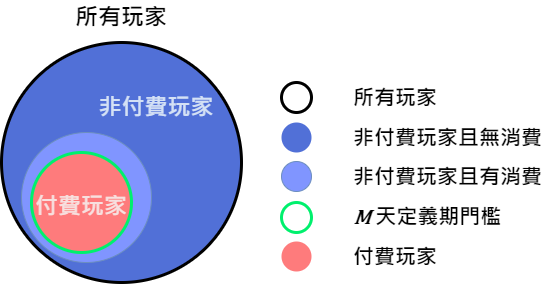
\includegraphics[width=0.5\textwidth]{figures/Image_ClassVennChart.png}
    \caption[流失玩家與非流失玩家范氏圖]{流失玩家與非流失玩家范氏圖}
    \label{fig:Image_ClassVennChart}
  \end{center}
\end{figure}

\subsection{資料特徵探勘與特徵工程}
\label{subsec:FeatureMining}

此步驟將探勘供機器學習使用之資料特徵。在遊戲領域巨量資料中,相較於在學習模型上進行深入研究與改進,透過資料特徵之轉化及選擇顯得更為重要且有效。所以對資料集進行不同面向之探勘,除了可以獲取更多的資訊,也能讓後續資料分析以及機器學習更加順利。

本文將觀察期作為資料特徵探勘期,對每位玩家進行資料特徵探勘。資料特徵之探勘面向將參考於~\cite{sifa2015predicting}~\cite{lee2016predicting}~\cite{martinez2020machine}之探勘想法,主要聚焦於玩家之行為軌跡,並將其進行特徵工程與設計綜合指標特徵。

圖~\ref{fig:Image_FeatureEngineering} 為特徵工程示意圖。紅色箭頭為第一層特徵變數建立方式,對資料集以多種統計方式建立資料特徵,並用多個時間框架做拆分,以獲得第一層特徵變數;藍色箭頭為第二層特徵變數建立方式,針對第一層特徵變數做計算,進一步來得到第二層特徵變數,如變化量特徵等。

\begin{figure}[!htb]
  \begin{center}
    
\includegraphics[width=0.95\textwidth]{figures/Image_FeatureEngineering.png}
    \caption[特徵工程示意圖]{特徵工程示意圖}
    \label{fig:Image_FeatureEngineering}
  \end{center}
\end{figure}
\newpage

最終可以將資料特徵種類分為三大類:

\begin{itemize}
  \item[■] 玩家輪廓資料:包含玩家自身相關資訊。如創帳號國家、玩家等級等。
  \item[■] 玩家平台操作紀錄:包含玩家以平台為探勘範疇之行為軌跡。如消費紀錄、客訴紀錄等。
  \item[■] 玩家遊戲行為軌跡:包含玩家以遊戲為探勘範疇之行為軌跡。如押注次數、贏分等。
\end{itemize}

\section{資料分析階段}

此階段將著重於資料的分析。為求在訓練機器學習前,可以藉由資料分析之方法來了解到資料之特性,以提高後續解讀資料特徵之重要性與其相關之連結。另外,還觀察資料特徵是否可以提供給學習模型較多的資訊。

\subsection{探索性資料分析}
採用探索性資料分析,藉由圖表呈現協助了解資料之特性,並且檢查高資訊量之資料特徵,此步驟將利用下列兩種圖表來觀察資料特性:

\begin{itemize}
  \item [■] 長條圖:比較資料數值,如圖~\ref{fig:Image_EDADiagrams} (a)。
  \item [■] 直方圖:觀察資料分布情況,如圖~\ref{fig:Image_EDADiagrams} (b)。
\end{itemize}

\begin{figure}[!htb]
  \centering
  \subfigure[長條圖] {
    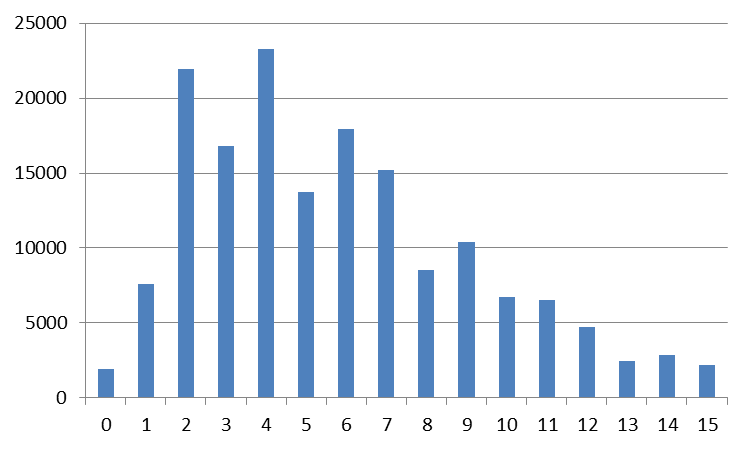
\includegraphics[width=0.45\columnwidth]{figures/Image_BarDiagram.png}
  }
  \subfigure[直方圖] {    
	  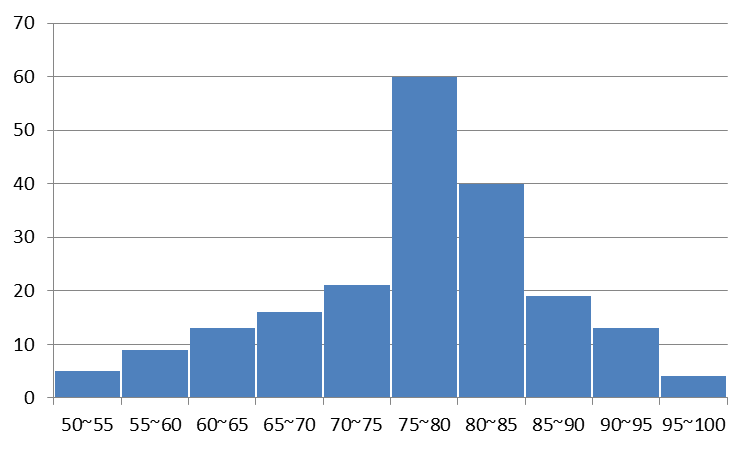
\includegraphics[width=0.45\columnwidth]{figures/Image_HistogramDiagram.png}
  }
  \caption[探索性資料分析之使用圖表類型]{探索性資料分析之使用圖表類型}
  \label{fig:Image_EDADiagrams}
\end{figure}

\subsubsection{高資訊量之資料特徵}
\label{subsubsec:ValuableFeatures}

藉由觀察資料特徵之分佈是否有明顯差異性,而推測此資料特徵能夠提供給學習模型較多的資訊,將此類資料特徵認為是高資訊量之資料特徵,使得後續資料特徵重要性分析之解釋可以更加順利。

假設玩家於觀察期間登入天數之人數統計如圖~\ref{fig:Image_ValuableFeatures},假設觀察期為4天。可以從圖中看出,非流失玩家數會隨著登入天數增加而遞增;流失玩家數則隨著登入天數增加而遞減,能夠容易地區分出流失玩家與非流失玩家,屬於高資訊量之資料特徵。

\begin{figure}[!htb]
  \begin{center}
    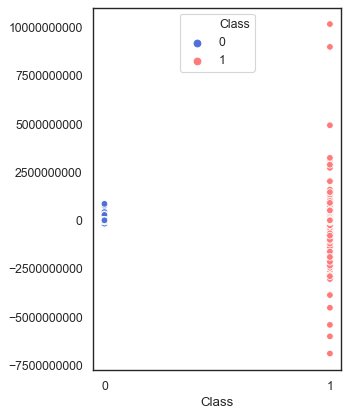
\includegraphics[width=0.55\textwidth]{figures/Image_ValuableFeatures.png}
    \caption[高資訊量之資料特徵示意圖]{高資訊量之資料特徵示意圖}
    \label{fig:Image_ValuableFeatures}
  \end{center}
\end{figure}

假設玩家於觀察期間登入天數之人數統計如圖~\ref{fig:Image_WorthlessFeatures},假設觀察期為4天。可以從圖中看出,無論是非流失玩家還是流失玩家,玩家數都隨著登入天數增加而遞增,較難以區分出流失玩家與非流失玩家,屬於低資訊量之資料特徵。

\begin{figure}[!htb]
  \begin{center}
    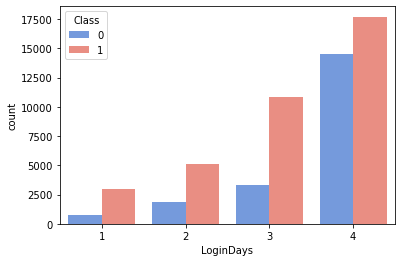
\includegraphics[width=0.55\textwidth]{figures/Image_WorthlessFeatures.png}
    \caption[低資訊量之資料特徵示意圖]{資訊量之資料特徵示意圖}
    \label{fig:Image_WorthlessFeatures}
  \end{center}
\end{figure}

\section{機器學習階段}
\label{sec:MachineLearning}

此階段將著重於機器學習訓練以及不平衡資料權重調整,最後產出最佳模型之預測結果,提供給流失玩家之預測分析以及資料特徵重要性分析使用。本文選擇樹狀結構之學習模型進行訓練,樹狀結構之學習模型對於巨量資料分類預測顯得更為合適,並且對於預測結果之解釋也相對清楚,而本論文所挑選之學習模型包含:決策樹、隨機森林與極限梯度提升。

\subsection{分割訓練與測試資料集}
\label{subsec:SplitDataset}

透過前述 \ref{subsec:DataFilter}~小節過濾後之資料集,進行訓練集與測試集分割,並按照 $X$:$Y$ 之比例隨機分配。為了避免隨機切割時,目標類別分布不平衡,將採分類隨機抽樣,即流失玩家與非流失玩家各別以 $X$:$Y$ 之比例隨機抽樣,如圖~\ref{fig:Image_SplitDataset}。

\begin{figure}[!htb]
  \begin{center}
    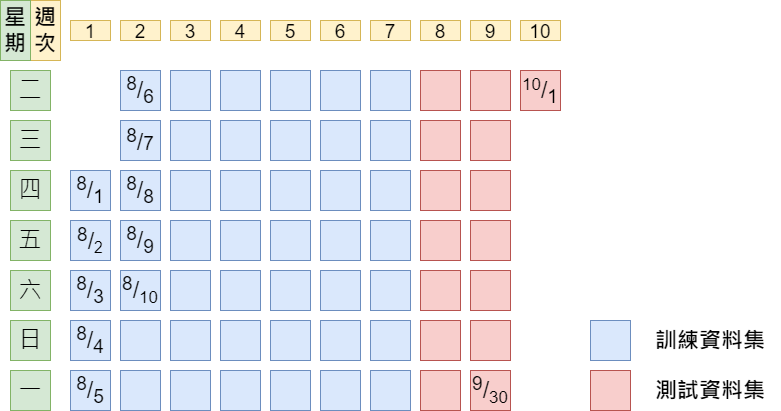
\includegraphics[width=0.8\textwidth]{figures/Image_SplitDataset.png}
    \caption[分割訓練與測試資料集示意圖]{分割訓練與測試資料集示意圖 (以$X$、$Y$分別為 8、2 為例) }
    \label{fig:Image_SplitDataset}
  \end{center}
\end{figure}

\subsection{學習模型選擇}
\label{subsec:ModelSelection}

本文選擇樹狀結構的學習模型進行訓練。樹狀結構的學習模型對於巨量資料分類預測顯得更為合適,並且對於預測結果之解釋也相對清楚,是研究中常使用的學習模型~\cite{wu2008top},因其模型結構能夠清楚表現每筆樣本之預測路徑,可以協助了解到學習模型如何做出決策,如白箱模型 ( white box model );而神經網路結構之學習模型,其模型內的結構難以解析,如黑箱模型 ( black box model ),則無法進行更一步的研究。而本論文所挑選之學習模型包含:
\newpage

\begin{itemize}
  \item [■] 決策樹:樹狀結構學習模型之最基礎結構,單樹結構,採用CART ( Classification and Regression Tree ) 演算法進行建樹。
  \item [■] 隨機森林:多樹結構,採用裝袋算法建樹。
  \item [■] 極限梯度提升:多樹結構,採用提升方法建樹。
\end{itemize}

上述三種學習模型之資訊量計算以基尼不純度 ( Gini Impurity, $G$ ) 為主,如式~\ref{eq:GiniImpurityFormula},其中$c$為$Class$、$p(i)$為$c$之發生機率。透過基尼不純度 ( $G$ ) 來衡量建樹時之分類準則,挑選出最適合用來進行分割之資料特徵及數值。

\begin{equation}
  \label{eq:GiniImpurityFormula}
  Gini\ Impurity(D) = G(D) = 1 - \sum_{i = 1}^{c}\ p(i)^2
\end{equation}

最後將比較上述三種不同學習模型來挑選出最佳之模型,包含裝袋算法與提升方法不同方式之建樹差異。

\subsection{不平衡資料權重調整}
\label{subsec:ImbalancedDataHandle}

進行機器學習訓練於遊戲領域巨量資料時,往往將會遭受資料不平衡之問題,進而影響學習模型之成效與可靠度。

普遍研究中將針對資料集進行預處理, 設法解決資料不平衡之問題,如SMOTE,為了讓少數群之樣本數與多數群相等,會於原始資料集中放入模擬資料。但本文為了確保資料間之真實性,於處理不平衡資料時,不希望針對資料集進行加工,會無法呈現出真實資料集之特性,所以本文將重點放於訓練學習模型時的樣本權重影響,而不對資料集進行直接處理。樣本權重設置如式~\ref{eq:SampleWeightFormula},其中$N_0$為非流失玩家 ( $class\ 0$ )之樣本數;$N_1$為流失玩家 ( $class\ 1$ )之樣本數。將計算$N_0$與$N_1$之比例差距,此值則為非流失玩家 ( $class\ 0$ )樣本權重放大倍數。

\begin{equation}
  \label{eq:SampleWeightFormula}
%  class\ 0 : class\ 1 = \left \lfloor{\frac{N_1}{N_0}}\right \rfloor : 1
  class\ 0 : class\ 1 = \frac{N_1}{N_0} : 1
\end{equation}

\subsection{搜尋最佳參數解}
\label{subsec:TuningBestParams}

此步驟將對前述 \ref{subsec:ModelSelection}~小節挑選之學習模型進行搜尋最佳參數解,以調教出最適合該學習模型之參數。各學習模型之調教參數如表~\ref{tab:ModelParamsTuning},針對各學習模型之結構不同,挑選不同的參數進行最佳化,各參數意義說明如表~\ref{tab:ModelParamsDescription}。

\begin{table}[!htb]
	\centering
	\begin{tabular}{cclclcl}
		\hline \hline
		學習模型 && Decision Tree && Random Forest && XGBoost \\
    \hline \hline
    \multirow{4}*{參數調教} && max\char`_depth && n\char`_estimators && n\char`_estimators \\
    && min\char`_samples\char`_split && max\char`_depth && max\char`_depth \\
    && min\char`_samples\char`_leaf && min\char`_samples\char`_split && \\
    && min\char`_samples\char`_leaf &&&& \\
    \hline \hline
		\end{tabular}
	\caption[學習模型參數調教表]{學習模型參數調教表}
	\label{tab:ModelParamsTuning}
\end{table}

\begin{table}[!htb]
	\centering
	\begin{tabular}{ccl}
		\hline \hline
		參數 && 參數說明 \\
    \hline \hline
    n\char`_estimators && 多樹結構之樹總數 \\
    \hline
    max\char`_depth && 樹狀結構之最大深度限制 \\
    \hline
    min\char`_samples\char`_split && 節點分割之最小樣本數限制 \\
    \hline
    min\char`_samples\char`_leaf && 葉節點之最小樣本數限制 \\
    \hline \hline
		\end{tabular}
	\caption[學習模型參數說明表]{學習模型參數說明表}
	\label{tab:ModelParamsDescription}
\end{table}

\subsection{交叉驗證 ( Cross Validation ) }
\label{subsec:CrossValidation}

針對訓練資料集進行交叉驗證 ( Cross Validation ),並且搭配前頁之參數調教,最後輸出最佳模型。參考了~\cite{brownlee2020imbalanced}中所使用之RepeatedStratifiedKFold方法,其中使用Stratified方式分割,即為在各Fold中,流失玩家與非流失玩家之資料比例將會相等;使用Repeated方式反覆驗證,即為反覆執行上述之交叉驗證。透過上述之分割方式,可以在每次訓練學習模型時,使真實訓練集保持著原始訓練集的流失玩家與非流失玩家比例。

圖~\ref{fig:Image_RepeatedStratifiedKFold} 為RepeatedStratifiedKFold示意圖。可以從圖中看出,首先依照前述 \ref{subsec:SplitDataset}~小節,從所有資料初步分割出原始訓練集與測試集,再針對原始訓練集進行RepeatedStratifiedKFold,進行了兩次的交叉驗證,而每次分割原始訓練集時可以看到淺藍底之真實訓練集與淺橘底之驗證集中的流失玩家與非流失玩家比例與原始測試集相等,並且真實訓練集與驗證集中的流失玩家與非流失玩家比例也相等。

\begin{figure}[!htb]
  \begin{center}
    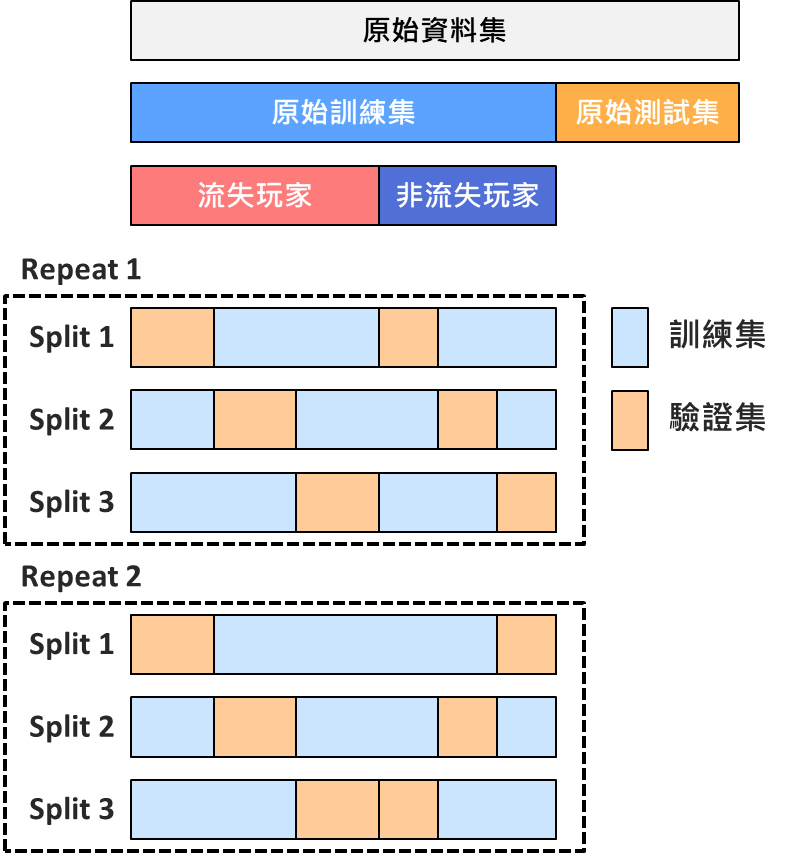
\includegraphics[width=0.65\textwidth]{figures/Image_RepeatedStratifiedKFold.png}
    \caption[RepeatedStratifiedKFold示意圖]{RepeatedStratifiedKFold示意圖 (以Repeated、KFold分別為 2、3 為例) }
    \label{fig:Image_RepeatedStratifiedKFold}
  \end{center}
\end{figure}

\subsection{評估驗證最佳模型}
\label{subsec:EvaluateBestModel}

前述 \ref{subsec:CrossValidation}~小節中,交叉驗證搭配 \ref{subsec:TuningBestParams}~小節中的參數調教表所使用之評估值為 Weighted F$_{\beta}$ - Score,擇其最高值之學習模型,選定為最佳模型。Weighted F$_{\beta}$ - Score 為在 F$_{\beta}$ - Score 評估值上導入樣本數權重概念,如式~\ref{eq:FbetaFormula} 與式~\ref{eq:WeightedFbetaFormula},適合使用在評估資料不平衡之資料集中。

\begin{equation}
  \label{eq:FbetaFormula}
  F_{\beta} = (1 + \beta^2) \times \frac{precision \times recall}{(\beta^2 \times precision) + recall}
\end{equation}

\begin{equation}
  \label{eq:WeightedFbetaFormula}
  Weighted\ F_{\beta} = \frac{N_1}{N_0 + N_1} \times F_{\beta\ 1} + \frac{N_0}{N_0 + N_1} \times F_{\beta\ 0}
\end{equation}

其中 $\beta$ 則為 Precision 與 Recall 之間的比重,如表~\ref{tab:beta}。本論文預測新進玩家是否會流失,將著重於 Recall,即為將所有可能流失的新進玩家預測出來,因為新進玩家有可能是經由廣告吸引而來,而該玩家身上即帶有廣告投放之成本,故希望能將有可能會流失的新進玩家全部預測出來,使得遊戲商能盡可能地保留住所有玩家。

\begin{table}[!htb]
	\centering
	\begin{tabular}{ccl}
		\hline \hline
		$\beta$數值範圍 && 說明 \\
    \hline \hline
    $0 < \beta < 1$ && 評估著重於 Precision \\
    \hline
    $\beta = 1$ && Precision 與 Recall 比重相當 \\
    \hline
    $1 < \beta$ && 評估著重於 Recall \\
    \hline \hline
		\end{tabular}
	\caption[$\beta$數值意義表]{$\beta$數值意義表}
	\label{tab:beta}
\end{table}

\section{預測結果分析階段}
\label{sec:PredictionResultAnalysis}

此階段將著重於資料特徵重要性之分析。透過前述 \ref{subsec:EvaluateBestModel}~小節所產出之預測結果,計算其資料特徵於各學習模型中各樹之重要性,並加總後正規化,產出之分析結果將與前述 \ref{subsubsec:ValuableFeatures}~小節中推測之資料特徵進行探討,並藉由最終結果對遊戲中的遊玩體驗進行評估與建議。

\subsection{資料特徵重要性分析}
\label{subsec:FeatureImportanceAnalysis}

將資料特徵重要性 ( Feature Importance, $fi$ ) 定義為加總各樹中各資料特徵於節點分割時所提供之基尼不純度 ( $G$ ) ( 見式~\ref{eq:GiniImpurityFormula} ) ,稱為基尼重要性 ( Gini Importance, $GI$ ),再將其正規化至區間[0,1]中。

式~\ref{eq:GiniImportanceFormula} 為計算樹中各節點之基尼重要性 ( $GI$ ),其中$D_p$為父節點、$N_p$為父節點之樣本數、$D_{left}$為左子節點、$N_{left}$為左子節點之樣本數、$D_{right}$為右子節點、$N_{right}$為右子節點之樣本數。首先計算$D_p$、$D_{left}$及$D_{right}$之基尼不純度 ( $G$ ),並計算$D_{left}$及$D_{right}$之樣本數權重比例,最後將$D_p$之基尼不純度 ( $G$ ) 減去兩權重值。

\begin{equation}
  \label{eq:GiniImportanceFormula}
  Gini\ Importance(D_p) = GI(D_p) = G(D_p) - \frac{N_{left}}{N_p} \times G(D_{left}) - \frac{N_{right}}{N_p} \times G(D_{right})
\end{equation}

式~\ref{eq:SingleTreeFeatureImportanceFormula} 為計算資料特徵於單樹中之重要性,其中$x$為欲求其重要性之資料特徵、$k$為節點分割時所用資料特徵為$x$之所有節點、$l$為樹中所有節點。首先加總所有$k$之基尼重要性 ( $GI$ ),並加總$l$之基尼重要性 ( $GI$ ),最後將其進行正規化計算,落於區間[0,1]中,並總和為1。

\begin{equation}
  \label{eq:SingleTreeFeatureImportanceFormula}
  fi(t,x) = \frac{\sum_{\ k\ \in\ node\ split\ based\ on\ x}GI(D_k)}{\sum_{\ l\ \in\ all\ nodes}GI(D_l)}
\end{equation}

式~\ref{eq:ModelFeatureImportanceFormula} 為計算資料特徵於多樹中之重要性,其中$x$為欲求其重要性之資料特徵、$t$為學習模型中的所有樹、$N_{trees}$為樹總數。首先加總所有$t$中$x$的$fi(t,x)$,並取其平均於$N_{trees}$中,最後即計算出$x$於學習模型內之資料特徵重要性 ( $fi$ ) 。

\begin{equation}
  \label{eq:ModelFeatureImportanceFormula}
  fi(x) = \frac{\sum_{\ t\ \in\ all\ trees}fi(t,x)}{N_{trees}}
\end{equation}

\section{產業應用分析階段}
\label{sec:ApplicationAnalysis}

此階段將著重於建立代理人模型。代理人模型為一種優化方法,當模型較為複雜、計算量較大時,可以用一簡化模型來替代,如決策樹‧

\subsection{代理人模型}
\label{subsec:SurrogateModel}

圖~\ref{fig:Image_SurrogateModel} 為代理人模型示意圖,用決策樹作為極限梯度提升之代理人模型,結構上較為簡單,在解釋玩家流失的行為規則上也較為清楚,讓市場操作人員的挽留策略更加明確。

\begin{figure}[!htb]
  \begin{center}
    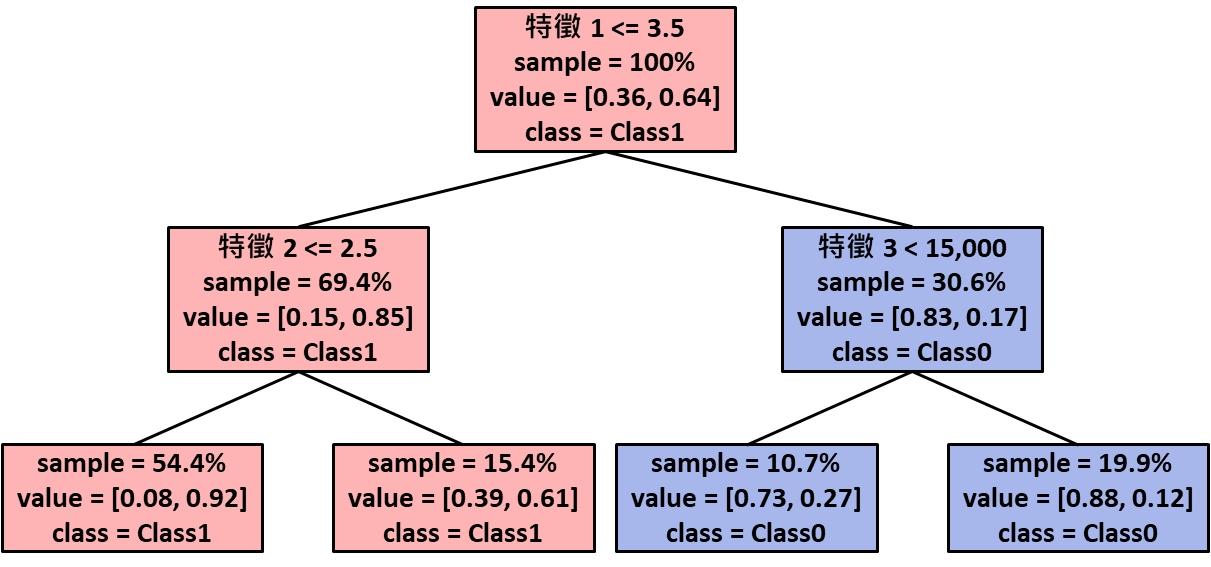
\includegraphics[width=0.85\textwidth]{figures/Image_SurrogateModel.png}
    \caption[代理人模型示意圖]{代理人模型示意圖}
    \label{fig:Image_SurrogateModel}
  \end{center}
\end{figure}
\newpage
%%% 	\chapter{實驗結果與分析}
\label{cha:Evaluation}

此章節中,我們將針對前述第~\ref{cha:Method}~章之研究方法進行實驗結果評估與分析,第~\ref{sec:SystemStructure}~小節說明實驗系統架構、第~\ref{sec:DataPreprocessEvaluation}~小節說明資料前處理評估、第~\ref{sec:DataAnalysisEvaluation}~小節說明資料分析評估、第~\ref{sec:MachineLearningEvaluation}~小節說明機器學習評估、第~\ref{sec:PredictionResultAnalysisEvaluation}~小節說明預測結果分析評估,以及第~\ref{sec:ApplicationAnalysisEvaluation}~小節說明產業應用分析評估。

\section{實驗系統架構}
\label{sec:SystemStructure}

本論文實驗系統架構將分為資料前處理端、資料分析端與機器學習端,如~\ref{tab:ResearchEnvironment},並均以 Python 3.9.7 做為開發語言。

\begin{itemize}
    \item [■] 資料前處理端:以 Apache Spark 3.2.1~\cite{armbrust2015spark}處理資料之前處理以及分割資料集所使用。
    \item [■] 資料分析端:以 missingno 0.5.1~\cite{Bilogur2018}、Seaborn 0.11.2~\cite{michael_waskom_2020_3767070}協助以圖表方式呈現資料特性。
    \item [■] 機器學習端:以 pandas 1.3.4~\cite{jeff_reback_2020_3715232}~\cite{mckinney-proc-scipy-2010}、scikit-learn 0.24.2~\cite{scikit-learn}~\cite{sklearn_api}、XGBoost 1.6.1~\cite{chen2016xgboost}處理機器學習訓練與評估。
\end{itemize}

\begin{table}[!htb]
	\centering
	\begin{tabular}{cclclcl}
	\hline \hline
	系統端點 && 資料前處理端 && 資料分析端 && 機器學習端 \\
    \hline \hline
    \multirow{3}*{研究環境} && \emph{Apache Spark} && \emph{missingno} && \emph{pandas} \\
    &&&& \emph{Seaborn} && \emph{scikit-learn} \\
    &&&&&& \emph{XGBoost} \\
    \hline \hline
	\end{tabular}
	\caption[實驗系統架構之研究環境表]{實驗系統架構之研究環境表}
	\label{tab:ResearchEnvironment}
\end{table}

本文的資料集取自一博弈遊戲,此遊戲於全球發行,遊戲內容包含了老虎機 ( Fruit Machine )、魚機 ( Fish Hunter ) 和其他小遊戲。
\newpage

\section{資料前處理評估}
\label{sec:DataPreprocessEvaluation}

此階段將評估前章~\ref{sec:DataPreProcess} 小節之資料前處理。~\ref{subsec:AudienceEvaluation} 小節為預測受眾評估,將說明~\ref{subsec:DataFilter} 小節之資料過濾;~\ref{subsec:FeatureEvaluation} 小節為預測特徵評估,將說明~\ref{subsec:ClassPreparation} 小節之目標值準備及~\ref{subsec:FeatureMining} 小節之資料特徵探勘與特徵工程。

本文收集了 2022/03/01 至 2022/05/31 的資料,共計三個月。此資料集是以天為單位,記錄了玩家於遊戲平台上和各項遊戲內的行為軌跡。總容量約為 44 GB。

\subsection{預測受眾評估}
\label{subsec:AudienceEvaluation}

本文將日本新進玩家作為預測受眾,因為日本玩家相較於其他國家較少有不良的帳號紀錄\ (\ 例如:同一位玩家多次創建新帳號等\ ),其遊戲資料相對地會較有可信度。此外,本文特別排除了等級 10 以下的玩家,確保收集到的玩家資料皆是有通過新手教學的,讓後續產生的特徵更有價值。共有 60,469 位玩家作為預測受眾,來進行後續實驗。

接著進行資料過濾,以獲得有價值玩家。本文直接鎖定預測受眾於日本等級10以上之新進玩家,用到的資料集沒有空缺值存在,因此,會直接進行無價值玩家資料處理。本文根據市場操作人員的建議,將觀察期 ( $O$ )、挽留期 ( $R$ ) 及表現期 ( $P$ ) 分別設為 4 天、1 天及 2 天,將無價值玩家排除後,最後剩下 57,170 位有價值玩家,如表~\ref{tab:ValuePlayerObservation}。

\begin{table}[!htb]
	\centering
	\begin{tabular}{ccccc}
	\hline \hline
	新進玩家總數 & \tabincell{c}{日本等級10以上\\新進玩家數} & 空缺值玩家數 & 無價值玩家數 & 有價值玩家數 \\
    \hline \hline
    4,750,383 & 60,469 & 0 & 3,299 & 57,170 \\
    \hline
    \multicolumn{5}{c}{有價值玩家數 $=$ 日本等級10以上新進玩家數 $-$ 空缺值玩家數 $-$ 無價值玩家數} \\
    \hline \hline
	\end{tabular}
	\caption[有價值玩家觀察表]{有價值玩家觀察表}
	\label{tab:ValuePlayerObservation}
\end{table}
\newpage

\subsection{預測特徵評估}
\label{subsec:FeatureEvaluation}

圖~\ref{fig:eva_PlayerChurnPeriod} 為新進玩家之流失長條圖,用來觀察有價值玩家的流失速度。從圖中可以看出,隨著天數增加,有登入遊戲之玩家數量會跟著減少,創帳號後隔天有登入紀錄的玩家有 6 成左右,創帳號後第 3 天有登入紀錄者只剩下不到 4 成。故本論文聚焦於新進玩家之流失預測,希望能快速進行挽留策略,把握住新進玩家。

\begin{figure}[!htb]
    \begin{center}
      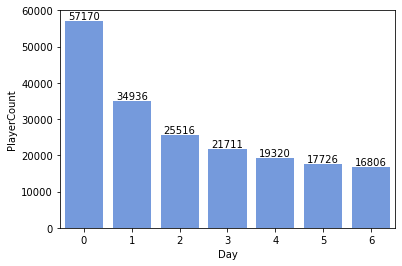
\includegraphics[width=0.7\textwidth]{figures/evaluation/Image_PlayerChurnPeriod.png}
      \caption[新進玩家之流失長條圖]{新進玩家之流失長條圖(x 軸為玩家登入日減去創立帳號日;y 軸為有登入之玩家數)}
      \label{fig:eva_PlayerChurnPeriod}
    \end{center}
\end{figure}

本文將定義新進玩家\ (\ 於~\ref{subsec:AudienceEvaluation}~小節中,篩選後之有價值玩家\ )\ 中的非流失玩家與流失玩家。觀察期有登入紀錄的玩家中,表現期間也有登入紀錄者視為非流失玩家,反之視為流失玩家。如表~\ref{tab:ChurnPlayerAndNonChurnPlayerDefinition},會有 20,488 位非流失玩家及 36,682 位流失玩家來做後續實驗。

\begin{table}[!htb]
	\centering
	\begin{tabular}{ccccc}
	\hline \hline
	有價值玩家數 & 非流失玩家 & 非流失玩家占比 & 流失玩家數 & 流失玩家占比 \\
    \hline \hline
    57,170 & 20,488 & 35.84 \% & 36,682 & 64.16 \% \\
    \hline \hline
	\end{tabular}
	\caption[非流失玩家及流失玩家定義表]{非流失玩家及流失玩家定義表}
	\label{tab:ChurnPlayerAndNonChurnPlayerDefinition}
\end{table}
\newpage

從原始資料集中探勘出$O$天\ (\ 資料特徵探勘期,即觀察期\ )\ 內之玩家資料,並以此來建立資料特徵。以計次、加總與平均,並以天為單位拆分時間段,產生第一層特徵變數,再對第一層特徵變數做計算,進而得到第二層特徵變數。最後,第一層特徵有156個,第二層特徵有93個,共得到了 249 個特徵變數。

另外,因類別型資料特徵不適用於樹狀結構之學習模型,故在其應用於機器學習前,將此類資料特徵透過 One Hot Encoding~\cite{wiki:OneHotEncoding}進行轉化,以利機器學習訓練,將此類特徵也歸類至第一層特徵,如圖~\ref{fig:eva_OneHotEncoder} 之作業系統。因此,第一層特徵數為 158 個,總特徵數為 251 個。

\begin{figure}[!htb]
    \begin{center}
      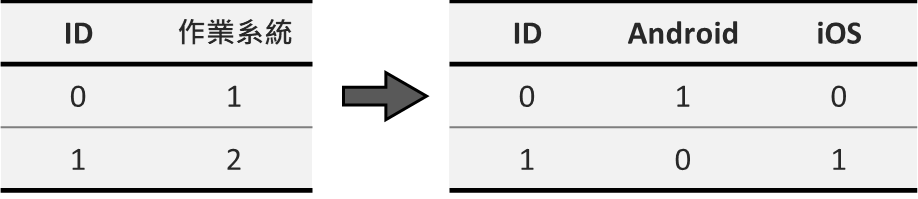
\includegraphics[width=0.75\textwidth]{figures/evaluation/Image_OneHotEncoder.png}
      \caption[作業系統 One Hot Encoding]{作業系統 One Hot Encoding (作業系統1為Android;2為iOS)}
      \label{fig:eva_OneHotEncoder}
    \end{center}
\end{figure}

為了避免特徵之間存在高度相關性,會影響到模型預測的準確性,本文對上述 251 個特徵變數進行篩選。透過支持向量機 ( Support Vector Machine ) 找出高共線性的冗贅特徵,並將其排除,最後只剩下 52 個特徵變數。此外,去掉高共線性的特徵也可以讓模型的可解釋性更好。表~\ref{tab:NumberOfFeatures} 為資料特徵總數表。圖~\ref{fig:eva_FirstFeatures} 為第一層變數圖、圖~\ref{fig:eva_SecondFeatures} 為第二層變數圖,而紅色底為篩選後之特徵。

\begin{table}[!htb]
	\centering
	\begin{tabular}{cccc}
	\hline \hline
	第一層特徵數 & 第二層特徵數 & 篩選前特徵數 & 篩選後特徵數 \\
    \hline \hline
    158 & 93 & 251 & 52 \\
    \hline \hline
	\end{tabular}
	\caption[資料特徵總數表]{資料特徵總數表}
	\label{tab:NumberOfFeatures}
\end{table}

為了避免部分特徵之數值過大或過小,彼此間差距較大,會影響到模型訓練精度,本文對所有特徵數值進行歸一化 ( Normalization )。式~\ref{eq:Normalization} 為本文歸一化的方式,會將所有數值映射到 [0,1] 區間。

\begin{equation}
  \label{eq:Normalization}
  x' = \frac{x-min(x)}{max(x)-min(x)}
\end{equation}
\newpage

\begin{figure}[!htb]
    \begin{center}
      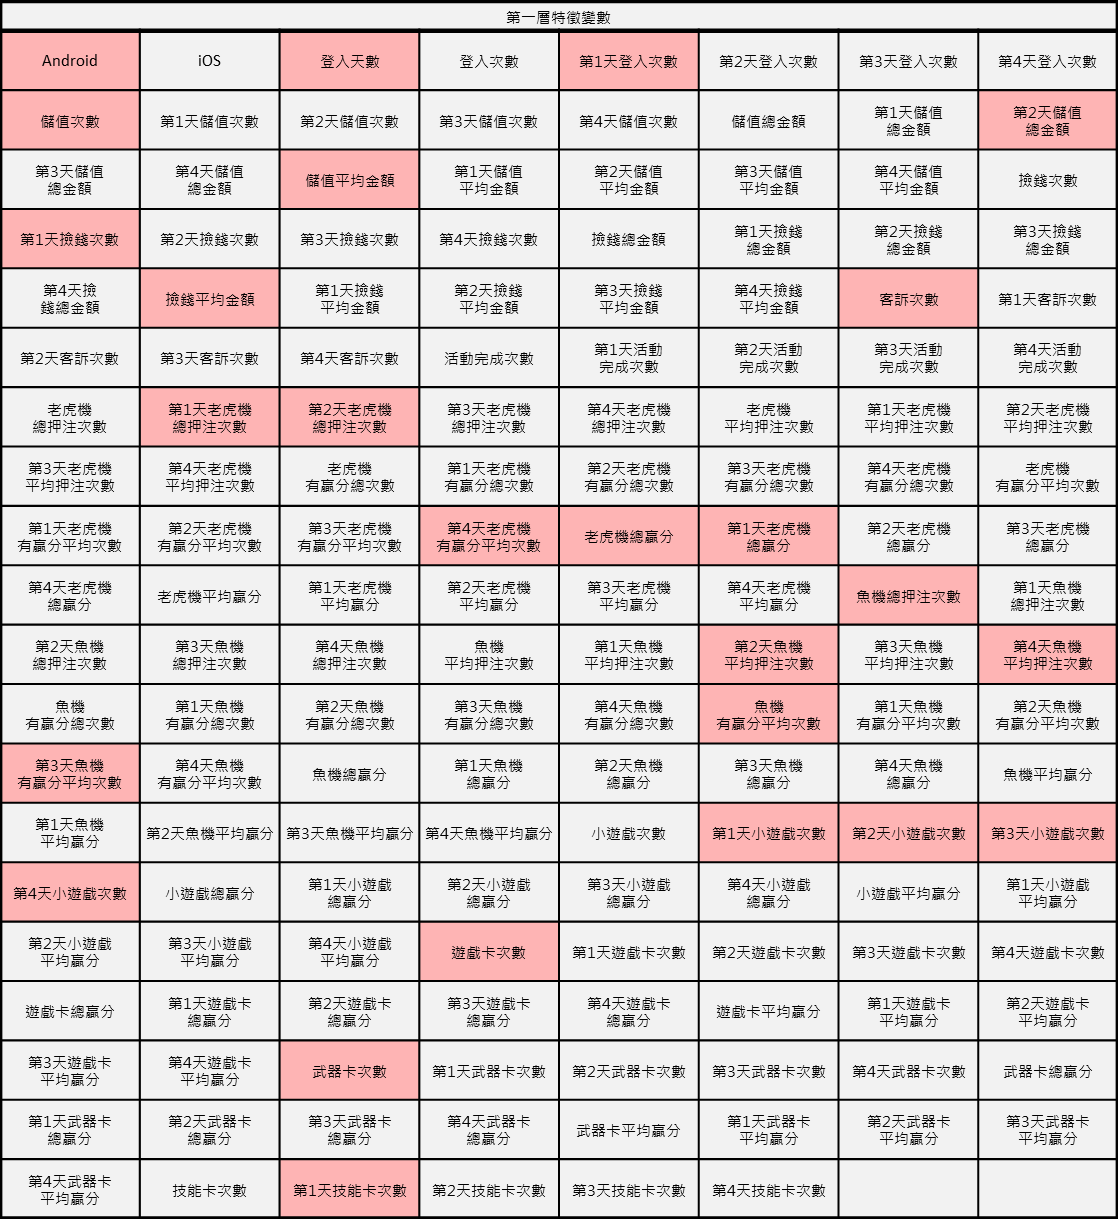
\includegraphics[width=1\textwidth]{figures/evaluation/Image_FirstFeatures.png}
      \caption[第一層特徵變數]{第一層特徵變數\ (\ 紅色底為篩選後之特徵\ )}
      \label{fig:eva_FirstFeatures}
    \end{center}
\end{figure}

\begin{figure}[!htb]
    \begin{center}
      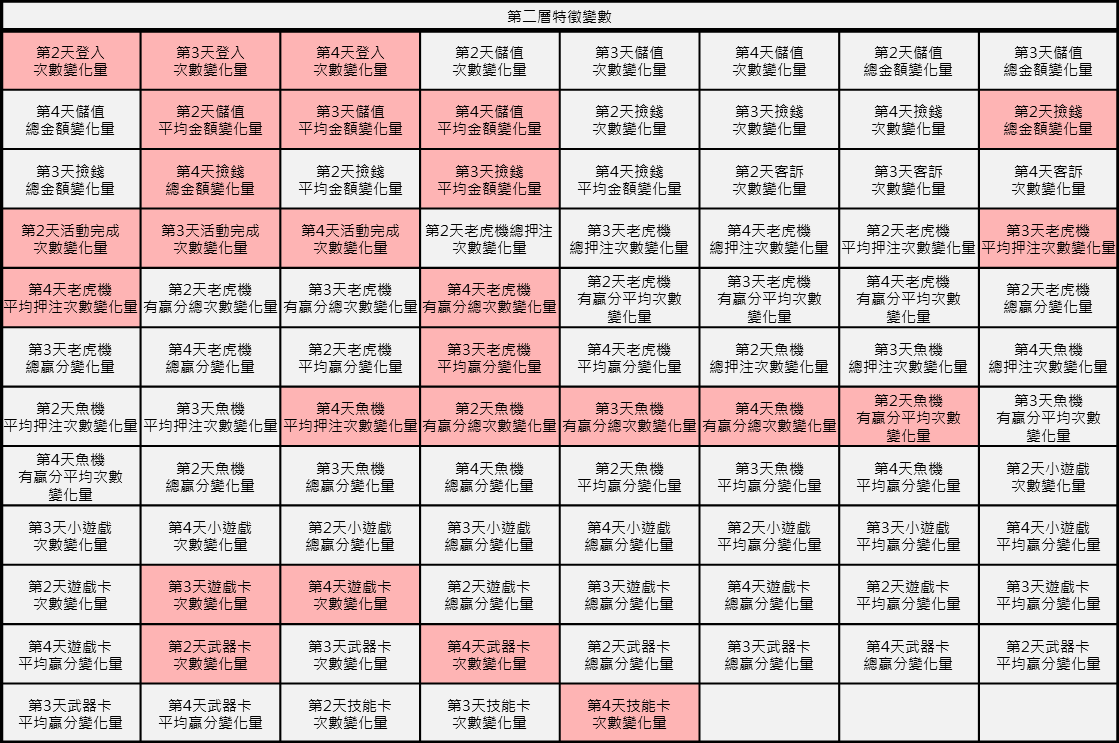
\includegraphics[width=1\textwidth]{figures/evaluation/Image_SecondFeatures.png}
      \caption[第二層特徵變數]{第二層特徵變數\ (\ 紅色底為篩選後之特徵\ )}
      \label{fig:eva_SecondFeatures}
    \end{center}
\end{figure}
\newpage

\section{資料分析評估}
\label{sec:DataAnalysisEvaluation}

此階段將評估前章 \ref{subsubsec:ValuableFeatures}~小節之高資訊量資料特徵推測,於 \ref{subsec:EDAEvaluation}~小節\ 探索性資料分析評估說明。

\subsection{探索性資料分析評估}
\label{subsec:EDAEvaluation}

利用長條圖及直方圖觀察在資料集中哪些特徵可能屬於高資訊量資料特徵。

圖~\ref{fig:eva_ValuableFeature_LoginDays} 為觀察期間玩家登入天數之人數統計圖。可以從圖中看出,非流失玩家數會隨著登入天數增加而遞增,流失玩家數則隨著登入天數增加而遞減。推測玩家登入天數可以帶給學習模型很好的分類資訊。

\begin{figure}[!htb]
    \begin{center}
      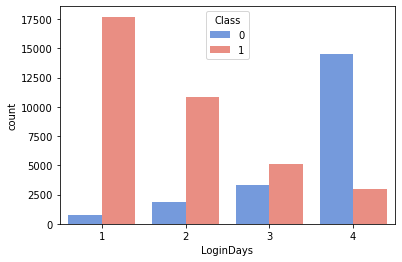
\includegraphics[width=0.7\textwidth]{figures/evaluation/Image_LoginDays.png}
      \caption[觀察期間玩家登入天數之人數統計圖]{觀察期間玩家登入天數之人數統計圖\ (\ x 軸為登入天數;y 軸為玩家數量\ )\ }
      \label{fig:eva_ValuableFeature_LoginDays}
    \end{center}
\end{figure}
\newpage

圖~\ref{fig:eva_ValuableFeature_DailyActivityMissionTimes} 為觀察期間玩家完成活動任務之次數統計圖。可以從圖中看出,除了創帳號當天以外,非流失玩家完成活動任務的次數皆遠大於流失玩家,甚至於創帳號後第三天,其次數變化量還為正值。推測活動任務完成次數之相關特徵可以帶給學習模型很好的分類資訊。

\begin{figure}[!htb]
    \begin{center}
      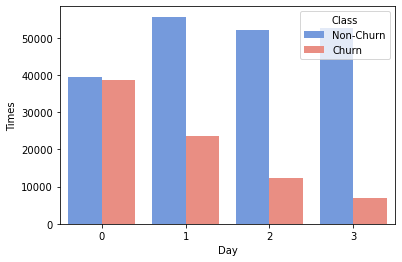
\includegraphics[width=0.7\textwidth]{figures/evaluation/Image_DailyActivityMissionTimes.png}
      \caption[觀察期間玩家完成任務之次數統計圖]{觀察期間玩家完成任務之次數統計圖\ (\ x 軸為觀察期第 x 天;y 軸為活動任務完成次數\ )\ }
      \label{fig:eva_ValuableFeature_DailyActivityMissionTimes}
    \end{center}
\end{figure}
\newpage

圖~\ref{fig:eva_ValuableFeature_D3SlotsMeanWinTimes} 為玩家創帳號後第三天之老虎機有贏分平均次數統計圖。可以從圖中看出,到了創帳號後第三天,流失玩家幾乎都沒有獲得贏分。推測此特徵可以帶給學習模型很好的分類資訊。

\begin{figure}[!htb]
    \begin{center}
      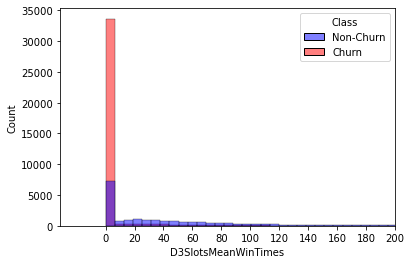
\includegraphics[width=0.7\textwidth]{figures/evaluation/Image_D3SlotsMeanWinTimes.png}
      \caption[玩家創帳號後第三天之老虎機有贏分平均次數統計圖]{玩家創帳號後第三天之老虎機有贏分平均次數\ (\ x 軸為平均有贏分次數;y 軸為玩家數量\ )\ (\ 紫色區域為非流失玩家與流失玩家重疊區域\ )\ }
      \label{fig:eva_ValuableFeature_D3SlotsMeanWinTimes}
    \end{center}
\end{figure}

圖~\ref{fig:eva_ValuableFeature_SystemType} 為作業系統各玩家統計圖。可以從圖中看出,不論是何種作業系統,流失玩家與非流失玩家的比例都差不多。推測作業系統的差異無法帶給學習模型很好的分類資訊。

\begin{figure}[!htb]
    \begin{center}
      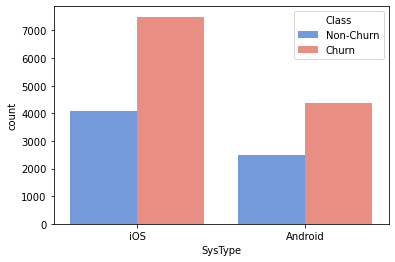
\includegraphics[width=0.7\textwidth]{figures/evaluation/Image_SystemType.png}
      \caption[作業系統各玩家統計圖]{作業系統各玩家統計圖\ (\ x 軸為作業系統;y 軸為玩家數量\ )\ }
      \label{fig:eva_ValuableFeature_SystemType}
    \end{center}
\end{figure}

\section{機器學習評估}
\label{sec:MachineLearningEvaluation}

此階段將評估前章~\ref{sec:MachineLearning} 小節之機器學習。~\ref{subsec:SplitDatasetEvaluation} 小節為分割訓練與測試資料集評估,將說明~\ref{subsec:SplitDataset} 小節之分割訓練與測試資料集;~\ref{subsec:ImbalancedDataHandleEvaluation} 小節為不平衡資料權重調整評估,將說明~\ref{subsec:ImbalancedDataHandle} 小節之不平衡資料權重調整;~\ref{subsec:BestModelEvaluation} 小節為最佳模型評估,將說明~\ref{subsec:TuningBestParams} 小節之搜尋最佳參數解及~\ref{subsec:EvaluateBestModel} 小節之評估驗證最佳模型;~\ref{subsec:TemporalWindowEvaluation} 小節為時間框架評估,將比較觀察期、表現期不同的天數,會對模型的輸出有甚麼影響。

\subsection{分割訓練與測試資料集評估}
\label{subsec:SplitDatasetEvaluation}

將資料集依照 8:2 之比例分割。如圖~\ref{fig:Image_SplitDataset},採分類隨機抽樣,即流失玩家與非流失玩家各別以 8:2 之比例隨機抽樣。表~\ref{tab:NumberOfSplitedPayerAndNonPayer} 為分割完資料集後之流失玩家數與非流失玩家數,訓練資料集與測試資料集之流失玩家與非流失玩家比例皆與原資料集相等,約為 1.79 倍。

\begin{table}[!htb]
	\centering
	\begin{tabular}{|c|r|r|}
	\hline \hline
	\diagbox{資料集}{玩家數} & 流失玩家 & 非流失玩家 \\
    \hline \hline
    訓練集 & 29,346 & 16,390 \\
    \hline
    測試集 & 7,336 & 4,098 \\
    \hline \hline
	\end{tabular}
	\caption[訓練與測試資料集玩家數表]{訓練與測試資料集玩家數表}
	\label{tab:NumberOfSplitedPayerAndNonPayer}
\end{table}

\subsection{資料不平衡處理評估}
\label{subsec:ImbalancedDataHandleEvaluation}

依照式~\ref{eq:SampleWeightFormula} 計算流失玩家樣本之縮小權重,如式~\ref{eq:SampleWeightCalculation},最後將流失玩家之樣本權重縮小 0.56 倍。

\begin{equation}
    \label{eq:SampleWeightCalculation}
    class\ 0 : class\ 1 = 1 : \frac{16,390}{29,346} = 1 : 0.56
\end{equation}
\newpage

圖~\ref{fig:eva_ROCCurveEvaluationImbalancedData} 為三種學習模型之ROC Curve,並比較不平衡資料處理前後之差異,(a)為決策樹、(b)為隨機森林、(c)為極限梯度提升,黃色線為未加入權重值、藍色線為加入權重值。從圖組中可以看出,在流失玩家之樣本權重上進行縮小,於本文並沒有明顯的作用,推測是因為本文預測的受眾資料並沒有極大的不平衡。

\begin{figure}[!htb]
    \centering
    \subfigure[決策樹ROC Curve圖] {
      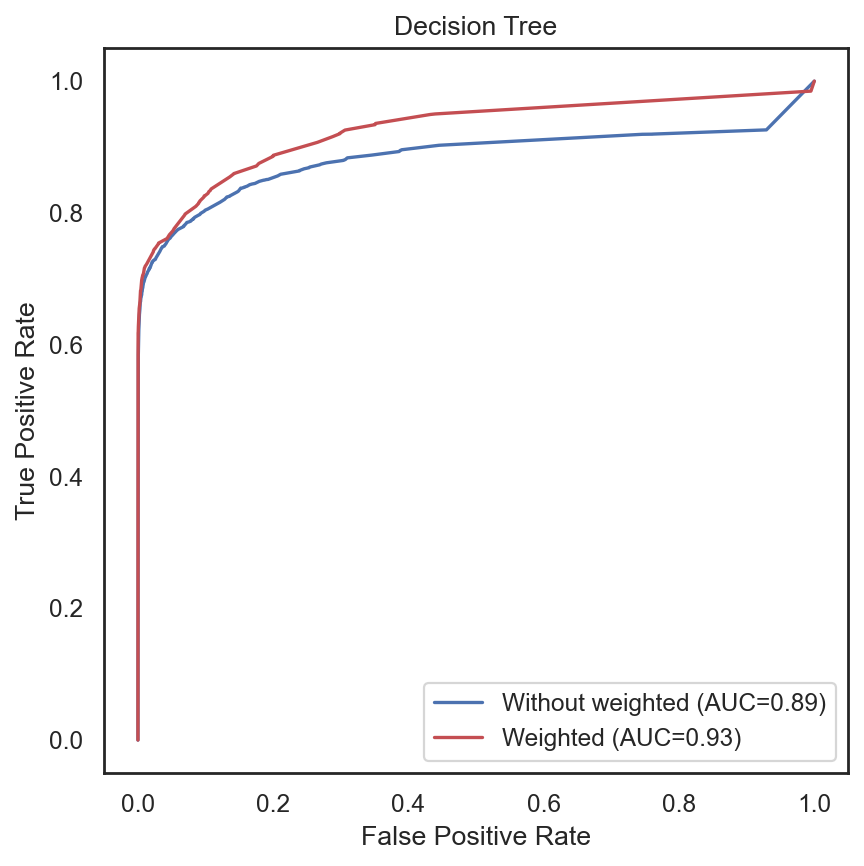
\includegraphics[width=0.47\columnwidth]{figures/evaluation/Image_DTROCCurve.png}
    }
    \subfigure[隨機森林ROC Curve圖] {
        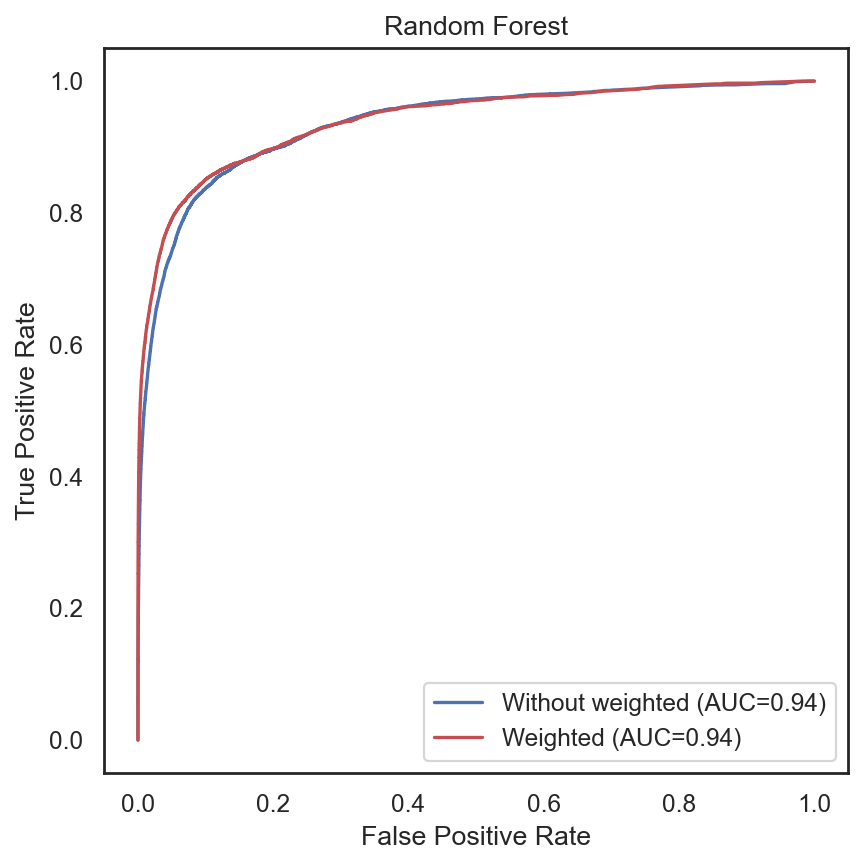
\includegraphics[width=0.47\columnwidth]{figures/evaluation/Image_RFROCCurve.png}
    }
    \subfigure[極限梯度提升ROC Curve圖] {
        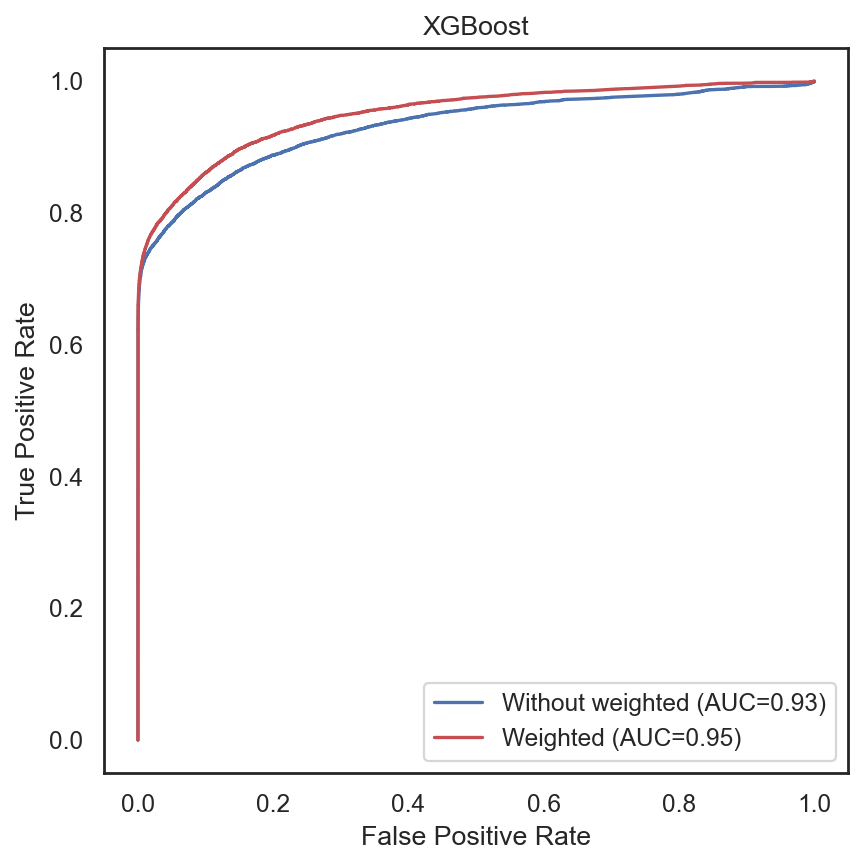
\includegraphics[width=0.47\columnwidth]{figures/evaluation/Image_XGBROCCurve.png}
    }
    \caption[不平衡資料處理前後比較之ROC Curve圖]{不平衡資料處理前後比較之ROC Curve圖\ (\ x 軸為假陽率;y 軸為真陽率\ )}
    \label{fig:eva_ROCCurveEvaluationImbalancedData}
\end{figure}
\newpage

圖~\ref{fig:eva_PRCurveEvaluationImbalancedData} 為三種學習模型之PR Curve,並比較不平衡資料處理前後之差異,(a)為決策樹、(b)為隨機森林、(c)為極限梯度提升,黃色線為未加入權重值、藍色線為加入權重值。從圖組中可以看出,在流失玩家之樣本權重上進行縮小,於本文並沒有明顯的作用,推測是因為本文預測的受眾資料並沒有極大的不平衡。

\begin{figure}[!htb]
    \centering
    \subfigure[決策樹PR Curve圖] {
      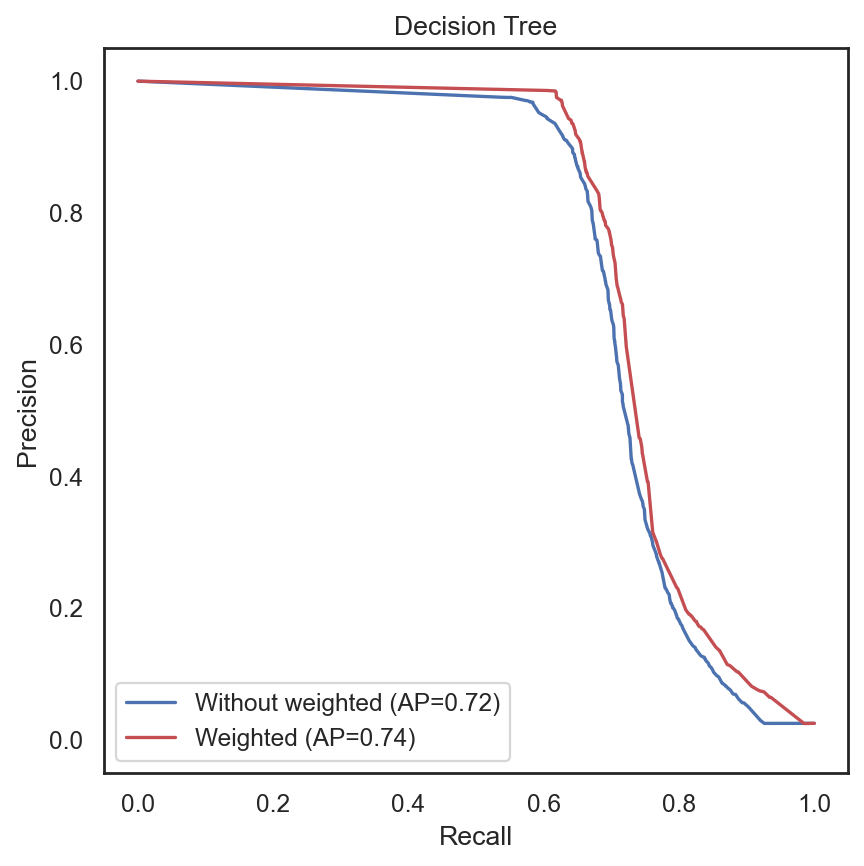
\includegraphics[width=0.47\columnwidth]{figures/evaluation/Image_DTPRCurve.png}
    }
    \subfigure[隨機森林PR Curve圖] {
        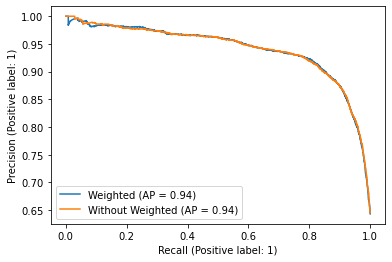
\includegraphics[width=0.47\columnwidth]{figures/evaluation/Image_RFPRCurve.png}
    }
    \subfigure[極限梯度提升PR Curve圖] {
        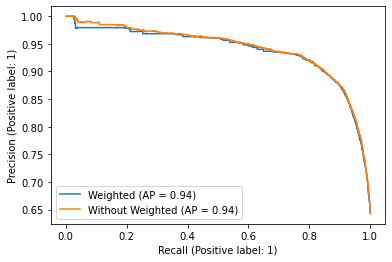
\includegraphics[width=0.47\columnwidth]{figures/evaluation/Image_XGBPRCurve.png}
    }
    \caption[不平衡資料處理前後比較之PR Curve圖]{不平衡資料處理前後比較之PR Curve圖\ (\ x 軸為召回率;y 軸為精確率\ )}
    \label{fig:eva_PRCurveEvaluationImbalancedData}
\end{figure}
\newpage

\subsection{最佳模型評估}
\label{subsec:BestModelEvaluation}

利用網格搜索與交叉驗證來調校出最佳模型。如圖~\ref{fig:Image_RepeatedStratifiedKFold},我們將採用Reapted 2次及5-Fold,最後使用測試資料集進行評估驗證,將說明 7,336 位流失玩家 ( $class\ 1$ ) 及 4,098 位非流失玩家 ( $class\ 0$ )。驗證結果如表~\ref{tab:BestModelEvaluation},從表中可以看出,極限梯度提升的結果表現為三種模型中最好的,因為其 Weighted F$_{\beta}$ - Score 為 0.849 是三者最高。

\begin{table}[!htb]
    \centering
        \begin{tabular}{|c|r|r|r|r|}
            \hline \hline
            \multirow{2}*{\diagbox{學習模型}{評估}} & $precision^+$ & $recall^+$ & ${F_{\beta}}^+$ & \multirow{2}*{$Weighted\ F_{\beta}$} \\
            \cline{2-4}
            & $precision^-$ & $recall^-$ & ${F_{\beta}}^-$ & \\
            \hline \hline
            \multirow{2}*{決策樹} & 0.892 & 0.863 & 0.870 & \multirow{2}*{0.846} \\
            \cline{2-4}
            & 0.769 & 0.813 & 0.802 & \\
            \hline
            \multirow{2}*{隨機森林} & 0.888 & 0.874 & 0.877 & \multirow{2}*{0.848} \\
            \cline{2-4}
            & 0.781 & 0.804 & 0.798 & \\
            \hline
            \multirow{2}*{極限梯度提升} & 0.887 & 0.876 & 0.878 & \multirow{2}*{0.849} \\
            \cline{2-4}
            & 0.783 & 0.801 & 0.796 & \\
            \hline
            \multicolumn{5}{|l|}{$+$:以正例(流失玩家 $class\ 1$ )為評估對象進行計算} \\
            \multicolumn{5}{|l|}{$-$:以反例(非流失玩家 $class\ 0$ )為評估對象進行計算} \\
            \hline \hline
        \end{tabular}
    \caption[最佳模型評估表]{最佳模型評估表}
    \label{tab:BestModelEvaluation}
\end{table}

圖~\ref{fig:eva_ModelsCurve} 為三種學習模型之曲線比較圖,(a) 為三種學習模型之ROC Curve比較圖、(b) 為三種學習模型之PR Curve比較圖,並且都為加入權重值之結果。從圖組中可以看出,隨機森林與極限梯度提升並沒有明顯的差異,原因可能在於特徵數量還不足夠,如果持續的擴增特徵,或許能凸顯出極限梯度提升的優點。

\begin{figure}[!htb]
    \centering
    \subfigure[三種學習模型之ROC Curve比較圖] {
      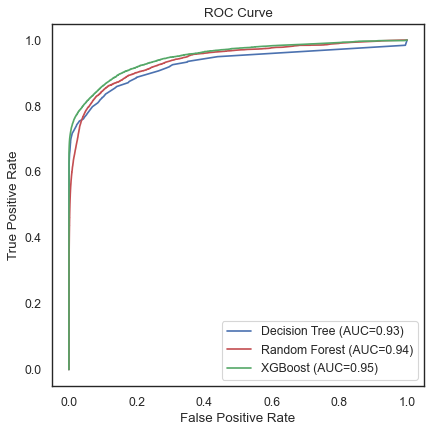
\includegraphics[width=0.48\columnwidth]{figures/evaluation/Image_ModelsROCCurve.png}
    }
    \subfigure[三種學習模型之PR Curve比較圖] {
        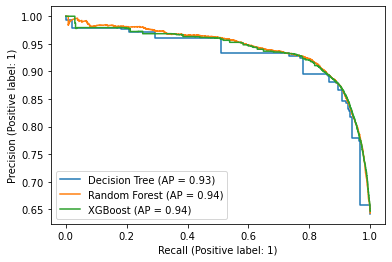
\includegraphics[width=0.48\columnwidth]{figures/evaluation/Image_ModelsPRCurve.png}
    }
    \caption[三種學習模型之曲線比較圖]{三種學習模型之曲線比較圖}
    \label{fig:eva_ModelsCurve}
\end{figure}

綜合上述得到的實驗結果,可以發現本文挑選的三種模型表現都不錯,Weighted F$_{\beta}$ - Score 都有接近 0.85,且曲線面積也都有 0.9 以上。可見本文建立的資料特徵能適用於各種模型中,並都有不錯的結果。

此外,極限梯度提升是採用梯度下降法 ( Gradient Descent ) 來加速學習模型之收斂,減少建樹時間成本,也較不會有過擬合 ( Overfitting ) 的情形出現。在訓練極限梯度提升模型時,可以將資料格式轉為極限梯度提升專用的 DMatrix 格式,以此來提升演算的效率。

表~\ref{tab:BestModelParams} 為三種學習模型之最佳參數解,參數搜尋範圍如表~\ref{tab:ParamsSearchRange}。決策樹因其為單樹結構,相較之下需要生成更深的樹;而隨機森林及極限梯度提升則因其為多樹結構,希望能以廣度發展,而非深度,相較之下需要生成更多的樹。

\begin{table}[!htb]
    \centering
        \begin{tabular}{clll}
            \hline \hline
            學習模型 & 決策樹 & 隨機森林 & 極限梯度提升 \\
            \hline \hline
            \multirow{4}*{參數調校} & max\char`_depth=5 & n\char`_estimators=60 & n\char`_estimators=25 \\
            & min\char`_samples\char`_split=2 & max\char`_depth=14 & max\char`_depth=5 \\
            & min\char`_samples\char`_leaf=20 & min\char`_samples\char`_split=6 & learning\char`_rate=0.05 \\
            && min\char`_samples\char`_leaf=5 & \\
            \hline \hline
        \end{tabular}
    \caption[最佳模型參數解表]{最佳模型參數解表}
    \label{tab:BestModelParams}
\end{table}

\begin{table}[!htb]
    \centering
        \begin{tabular}{cl}
            \hline \hline
            參數名 & 搜尋範圍 \\
            \hline \hline
            n\char`_estimators & 20, 25, 30, 35, 40, 45, 50, 55, 60 \\
            \hline
            max\char`_depth & 5, 6, 7, 8, 9, 10, 11, 12, 13, 14 \\
            \hline
            min\char`_samples\char`_split & 2, 4, 6, 8, 10 \\
            \hline
            min\char`_samples\char`_leaf & 1, 5, 10, 15, 20 \\
            \hline
            learning\char`_rate & 0.05, 0.07, 0.08, 0.1, 0.2 \\
            \hline \hline
        \end{tabular}
    \caption[參數搜尋範圍表]{參數搜尋範圍表}
    \label{tab:ParamsSearchRange}
\end{table}

\subsection{時間框架評估}
\label{subsec:TemporalWindowEvaluation}

將比較觀察期與表現期在不同天數的情況下,會對模型的輸出結果有甚麼影響,並用極限梯度提升來進行驗證。
\newpage

表~\ref{tab:BestObservationEvaluation} 為觀察期評估表,將挽留期及表現期設為1天及2天,並比較觀察期為2天、4天與6天的模型驗證結果。從表中可以看出,當觀察期越長時,模型的 Weighted F$_{\beta}$ - Score 越高,表示模型的表現結果越好。推測原因在於本文建立特徵的方式,因為能拆分更多的時間段,以此來獲得更多的玩家資料與特徵。

\begin{table}[!htb]
    \centering
        \begin{tabular}{|c|r|r|r|r|r|}
            \hline \hline
            \multirow{2}*{\diagbox{觀察期}{評估}} & $sample^+$ & $precision^+$ & $recall^+$ & ${F_{\beta}}^+$ & \multirow{2}*{$Weighted\ F_{\beta}$} \\
            \cline{2-5}
            & $sample^-$ & $precision^-$ & $recall^-$ & ${F_{\beta}}^-$ & \\
            \hline \hline
            \multirow{2}*{2天} & 6,570 & 0.834 & 0.767 & 0.790 & \multirow{2}*{0.780} \\
            \cline{2-5}
            & 4,905 & 0.718 & 0.796 & 0.766 & \\
            \hline
            \multirow{2}*{4天} & 7,336 & 0.887 & 0.876 & 0.878 & \multirow{2}*{0.849} \\
            \cline{2-5}
            & 4,098 & 0.783 & 0.801 & 0.796 & \\
            \hline
            \multirow{2}*{6天} & 7,701 & 0.913 & 0.907 & 0.908 & \multirow{2}*{0.878} \\
            \cline{2-5}
            & 3,589 & 0.803 & 0.815 & 0.813 & \\
            \hline
            \multicolumn{6}{|l|}{$+$:以正例(流失玩家 $class\ 1$ )為評估對象進行計算} \\
            \multicolumn{6}{|l|}{$-$:以反例(非流失玩家 $class\ 0$ )為評估對象進行計算} \\
            \hline \hline
        \end{tabular}
    \caption[觀察期評估表]{觀察期評估表}
    \label{tab:BestObservationEvaluation}
\end{table}

表~\ref{tab:BestPerformanceEvaluation} 為表現期評估表,將觀察期及挽留期設為4天及1天,並比較表現期為2天、4天與6天的模型驗證結果。從表中可以看出,當表現期越長時,模型的 Weighted F$_{\beta}$ - Score 越低,表示模型的表現結果越差。推測原因在於,定義是否流失的時間太長,原本會被定義為流失玩家的人,可能會變成非流失玩家,導致模型的預測能力受到影響。

\begin{table}[!htb]
    \centering
        \begin{tabular}{|c|r|r|r|r|r|}
            \hline \hline
            \multirow{2}*{\diagbox{表現期}{評估}} & $sample^+$ & $precision^+$ & $recall^+$ & ${F_{\beta}}^+$ & \multirow{2}*{$Weighted\ F_{\beta}$} \\
            \cline{2-5}
            & $sample^-$ & $precision^-$ & $recall^-$ & ${F_{\beta}}^-$ & \\
            \hline \hline
            \multirow{2}*{2天} & 7,336 & 0.887 & 0.876 & 0.878 & \multirow{2}*{0.849} \\
            \cline{2-5}
            & 4,098 & 0.783 & 0.801 & 0.796 & \\
            \hline
            \multirow{2}*{4天} & 6,779 & 0.867 & 0.845 & 0.852 & \multirow{2}*{0.828} \\
            \cline{2-5}
            & 4,449 & 0.773 & 0.802 & 0.793 & \\
            \hline
            \multirow{2}*{6天} & 6,463 & 0.849 & 0.846 & 0.847 & \multirow{2}*{0.821} \\
            \cline{2-5}
            & 4,548 & 0.782 & 0.786 & 0.785 & \\
            \hline
            \multicolumn{6}{|l|}{$+$:以正例(流失玩家 $class\ 1$ )為評估對象進行計算} \\
            \multicolumn{6}{|l|}{$-$:以反例(非流失玩家 $class\ 0$ )為評估對象進行計算} \\
            \hline \hline
        \end{tabular}
    \caption[表現期評估表]{表現期評估表}
    \label{tab:BestPerformanceEvaluation}
\end{table}
\newpage

從上述兩個表格中可以發現,當觀察期越長時,模型表現會越好,因為得到的特徵變多了;而當表現期越長時,模型表現會越差,因為原本該被定義為流失玩家的人,可能被定義成非流失玩家。但最後還是要根據市場需求來定義時間框架。

\section{預測結果分析評估}
\label{sec:PredictionResultAnalysisEvaluation}

此階段將評估前章~\ref{sec:PredictionResultAnalysis} 小節之預測結果分析。~\ref{subsec:FeatureImportanceEvaluation} 小節為資料特徵重要性評估,將說明~\ref{subsec:FeatureImportanceAnalysis} 小節之資料特徵重要性分析。

\subsection{資料特徵重要性評估}
\label{subsec:FeatureImportanceEvaluation}

將利用式~\ref{eq:GiniImportanceFormula}、式~\ref{eq:SingleTreeFeatureImportanceFormula} 及式~\ref{eq:ModelFeatureImportanceFormula} 計算之各資料特徵於各模型之資料特徵重要性。如圖~\ref{fig:eva_DTFeatureImportances}、圖~\ref{fig:eva_RFFeatureImportances} 及圖~\ref{fig:eva_XGBFeatureImportances},分別為決策樹、隨機森林及極限梯度提升之資料特徵重要性比較圖。

\begin{figure}[!htb]
    \begin{center}
      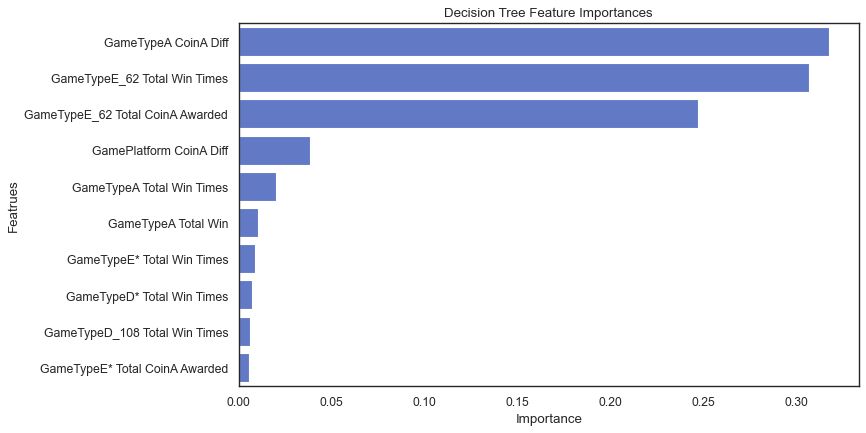
\includegraphics[width=1\textwidth]{figures/evaluation/Image_DTFeatureImportances.png}
      \caption[決策樹資料特徵重要性比較圖]{決策樹資料特徵重要性比較圖}
      \label{fig:eva_DTFeatureImportances}
    \end{center}
\end{figure}
\newpage

\begin{figure}[!htb]
    \begin{center}
      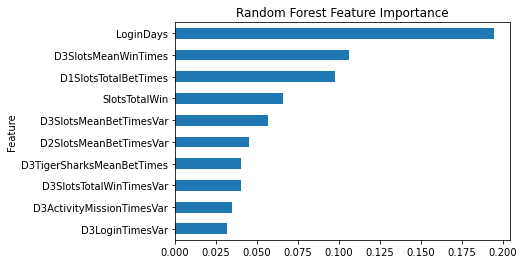
\includegraphics[width=1\textwidth]{figures/evaluation/Image_RFFeatureImportances.png}
      \caption[隨機森林資料特徵重要性比較圖]{隨機森林資料特徵重要性比較圖}
      \label{fig:eva_RFFeatureImportances}
    \end{center}
\end{figure}

\begin{figure}[!htb]
    \begin{center}
      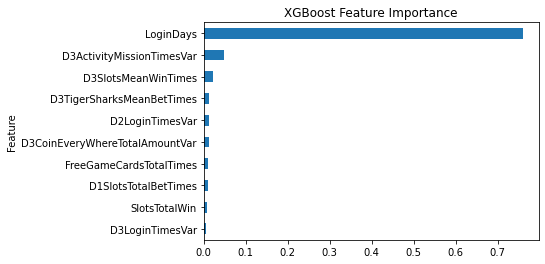
\includegraphics[width=1\textwidth]{figures/evaluation/Image_XGBFeatureImportances.png}
      \caption[極限梯度提升資料特徵重要性比較圖]{極限梯度提升資料特徵重要性比較圖}
      \label{fig:eva_XGBFeatureImportances}
    \end{center}
\end{figure}
\newpage

從三圖中可以看出,觀察期間的登入天數 ( LoginDays ) 皆是三種學習模型的第一名,可以說明登入天數的多寡確實與玩家是否流失有極大的關係。整合來看,在前十名中可以看到許多與變化量相關的特徵,如表~\ref{tab:FeatureImportanceTop10},雖不是主要原因,但可以從老虎機相關變化量特徵中說明,玩家是否流失確實與遊玩遊戲時的體驗起伏有關係。

\begin{table}[!htb]
    \centering
        \begin{tabular}{cl}
            \hline \hline
            參數名 & 代表意思 \\
            \hline \hline
            D2LoginTimesVar & 創帳號後第2天 登入次數變化量 \\
            \hline
            D3LoginTimesVar & 創帳號後第3天 登入次數變化量 \\
            \hline
            D2SlotsMeanWinVar & 創帳號後第2天 老虎機平均贏分變化量 \\
            \hline
            D2SlotsMeanBetTimesVar & 創帳號後第2天 老虎機平均押注次數變化量 \\
            \hline
            D3SlotsMeanBetTimesVar & 創帳號後第3天 老虎機平均押注次數變化量 \\
            \hline
            D3SlotsTotalWinTimesVar & 創帳號後第3天 老虎機有贏分總次數變化量 \\
            \hline
            D3ActivityMissionTimesVar & 創帳號後第3天 活動任務完成次數變化量 \\
            \hline
            D3CoinEveryWhereTotalAmountVar & 創帳號後第3天 撿錢總金額變化量 \\
            \hline \hline
        \end{tabular}
    \caption[特徵重要性前十名]{特徵重要性前十名\ (\ 變化量相關特徵\ )}
    \label{tab:FeatureImportanceTop10}
\end{table}

另外,三種學習模型之前十名資料特徵皆為數值型的資料特徵,而無類別型資料特徵,因其資料特徵重要性之評估以計算基尼重要性為主,數值型將會比類別型來得更為顯著,未來將可在計算重要性分析中,對於不同類型的資料特徵加入權重值,使得類別型的資料特徵能夠突出,讓整體分析更加準確。

\section{產業應用分析評估}
\label{sec:ApplicationAnalysisEvaluation}

此階段將評估前章~\ref{sec:ApplicationAnalysis} 小節之產業應用分析。~\ref{subsec:SurrogateModelEvaluation} 小節為代理人模型評估,將說明~\ref{subsec:SurrogateModel} 小節之代理人模型。

\subsection{代理人模型評估}
\label{subsec:SurrogateModelEvaluation}

代理人模型,以決策樹來說明極限梯度提升,能清楚地知道模型判斷是否流失的門檻,了解玩家流失的行為規則,在後續市場操作的策略上能有很好的建議。

圖~\ref{fig:eva_SurrogateModel} 為本文的代理人模型圖。從圖中來看,本文將數據集劃分為2個類別,即非流失玩家與流失玩家,其分別各占數據集的 0.36 與 0.64,所以最上面的根節點認為流失玩家的可能性較大。透過根節點可以知道,當玩家於觀察期間之登入天數\ (\ LoginDays\ )\ 小於 3 天時,有 69.4\% 的樣本數,且屬於流失玩家的可能性較大,因此會被判斷為流失玩家。繼續向下通過其他節點,分類結果就能更加確定。

此外,可以從代理人模型中發現,當登入天數小於 1 天時,流失機率已經高達 0.92。因此,可以建議遊戲商多推出留存規格,或是多舉辦與登入相關的活動,讓玩家增加其遊玩天數。

\begin{figure}[!htb]
    \begin{center}
      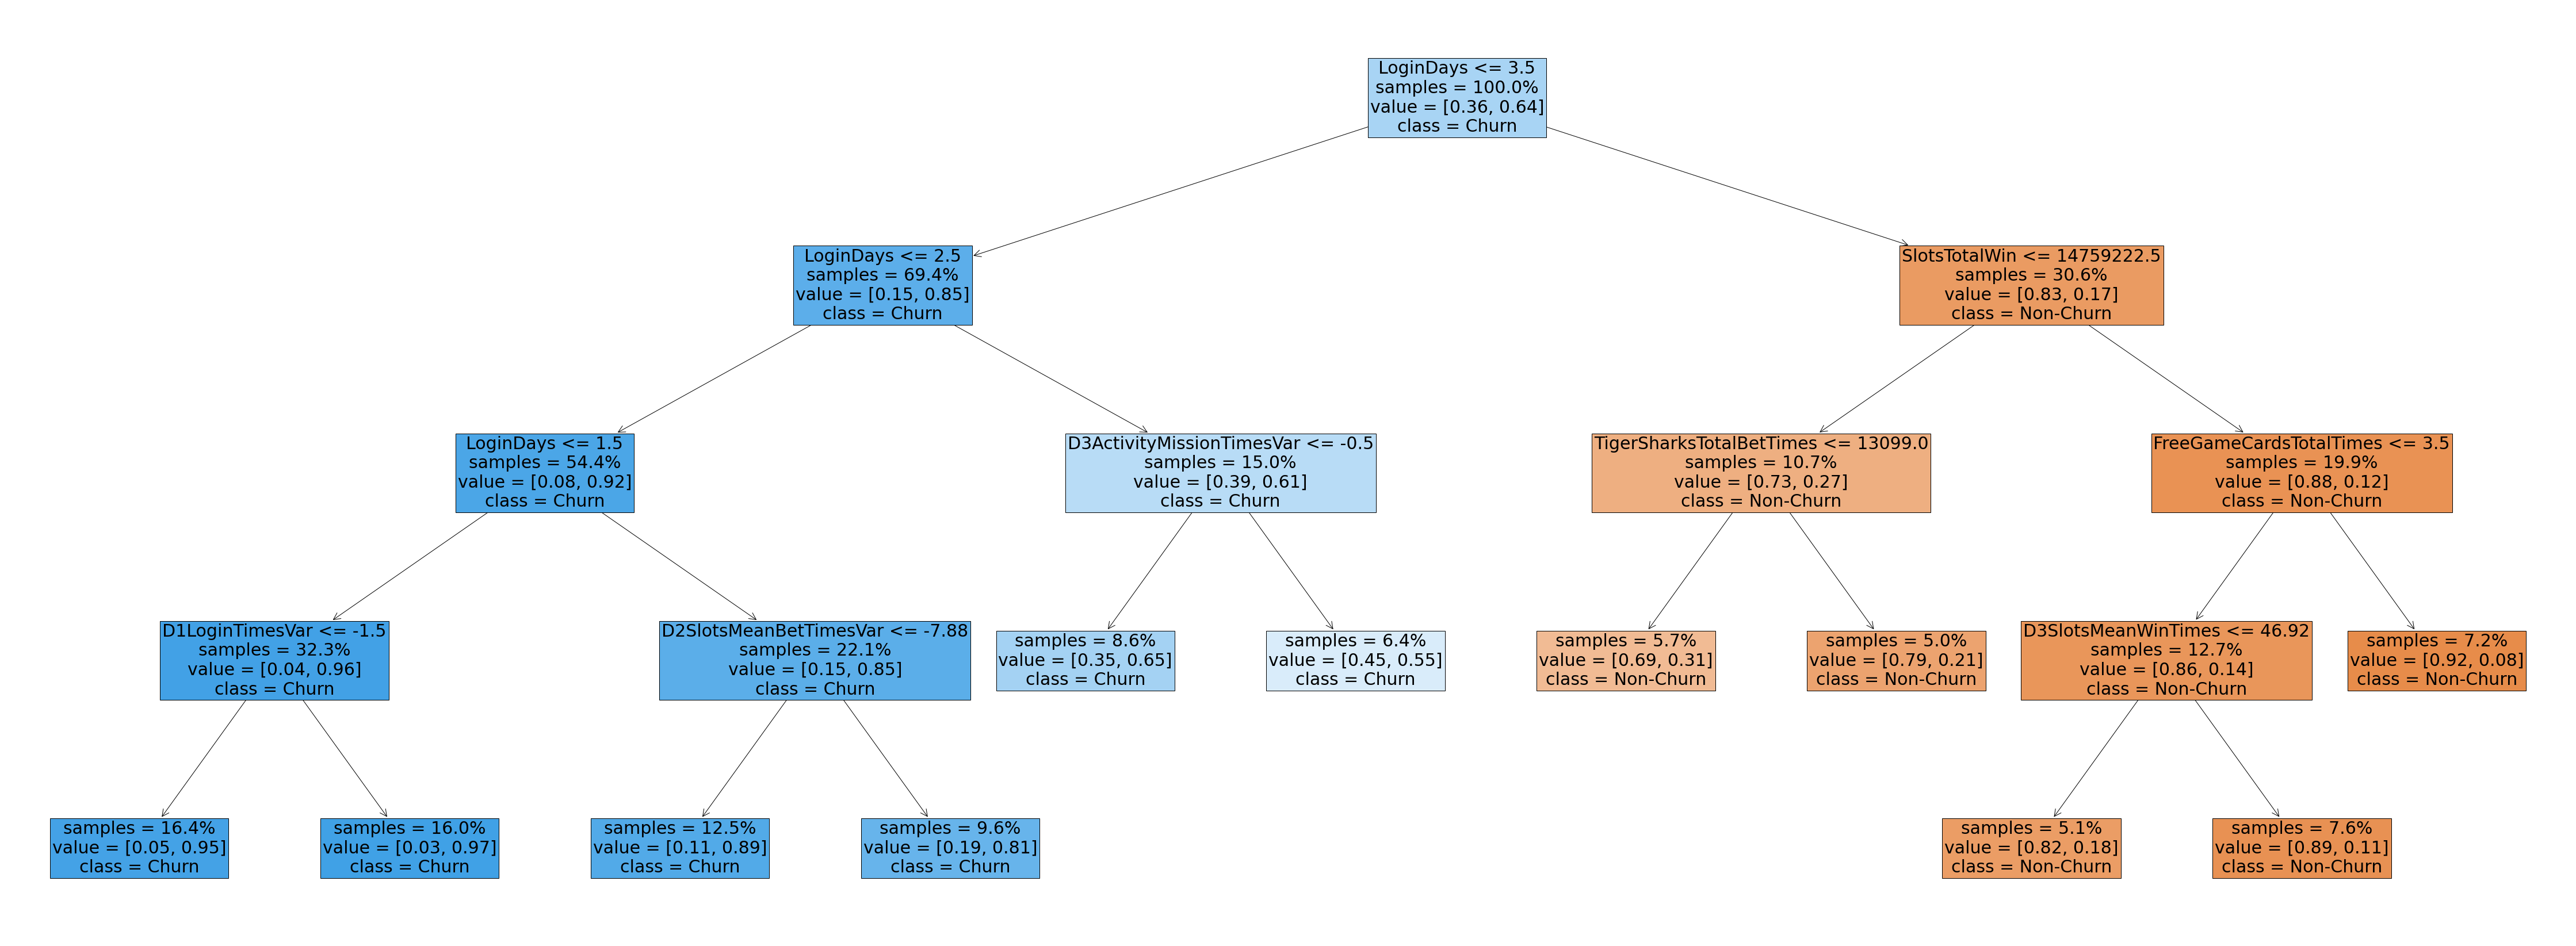
\includegraphics[width=1.5\textwidth, angle=90]{figures/evaluation/Image_SurrogateModel.png}
      \caption[代理人模型圖]{代理人模型圖}
      \label{fig:eva_SurrogateModel}
    \end{center}
\end{figure}
\newpage
%%% 	\chapter{結論與未來研究}
\label{cha:Conclusions}

\section{結論}

本論文提出一巨量資料探勘框架,框架拆分為四大階段進行,其中包括資料前處理、資料分析以及機器學習訓練等步驟。透過此框架可了解到資料前處理中的整合資料需求,並在清理資料時,過濾掉無價值的玩家,以提高整體分析成效,並且在目標值準備與資料特徵探勘時,給予一時間門檻,定義出合理的資料集,使得後續機器學習更加順利;藉由探索性資料分析處理資料集中不合適的資料特徵,並提早推測有助於遊戲平台發展的資料特徵;經由加入權重值於少數群,解決遊戲領域遭遇到的資料不平衡問題,而不透過修改原資料集的內容,再利用學習模型所輸出的預測結果,預測出付費玩家;最後以資料特徵重要性分析與藉由前述之推測,整理出資料特徵突出之原因,例如:玩家於遊戲體驗之起伏、玩家獲得獎勵或贏得遊戲所提高其付費意願。我們提出的框架可應用於遊戲領域且著重於新進玩家並經實驗證實,藉由前處理後的資料集,並同時針對資料不平衡進行處理,在預測潛在之新進付費玩家上有不錯的表現!並且我們可以進一步分析各資料特徵的重要性,協助解釋預測結果與遊戲內玩家行為軌跡的連動性,將可在遊戲平台行銷策略上提供意見,以更符合玩家真實環境所需,提高往後玩家之消費意願。

\section{未來研究}

由於本論文的資料特徵探勘種類受限於遊戲平台所提供的原始資料集,如能獲得更進一步的詳細資料,將可更加準確的預測出付費玩家。此外我們使用到的學習模型只有三種樹狀結構之模型,未來將可進行更多實驗於不同類型的學習模型,甚至導入時間序的概念,了解到玩家遊玩遊戲的順序差異是否會影響消費意願。最後除了可預測玩家是否會付費之外,未來還可進行付費時間點、購買商品種類等之預測,尚有許多議題可於遊戲領域巨量資料中研究。

	%----------------------------------------------------------------------------------------------------------------------------------------------------------
	% back pages 後頁
	% 包括參考文獻、附錄、自傳
	% 實際內容由
	%    my_bib.bib, my_appendix.tex, my_vita.tex
	% 決定
	% ntust_backpages.tex 此檔只提供整體架構的定義,不需更動
	% 在撰寫各章草稿時,可以把此部份「關掉」,以節省無謂的編譯時間。
	%
% this file is encoded in utf-8
% v1.7

%%% 參考文獻
\newpage
%\bibliographystyle{unsrt}
\phantomsection
\addcontentsline{toc}{chapter}{\nameRef}
\renewcommand{\bibname}{\protect\makebox[5cm][s]{\nameRef}}
%  \makebox{} is fragile; need protect
%\bibliographystyle{unsrt} 
\bibliographystyle{ieeetr}  % 使用 IEEE Trans 期刊格式
%\bibliographystyle{unsrt}
\bibliography{my_bib}  %reference 所需的bib檔
%\bibliographystyle{unsrt} 

%%% 附錄
%%
% this file is encoded in utf-8
% v1.7
%%% 每一個附錄 (附錄一、附錄二、...) 都要複製此段附錄編排碼做為起頭
%%% 附錄編排碼 begin >>>
\newpage
\chapter*{附錄一:MATLAB 程式列表} % 修改附錄編號與你的附錄名
\addcontentsline{toc}{chapter}{附錄一:MATLAB 程式列表} %建議此內容應與上行相同
\renewcommand{\thechapter}{一} % 如果是附錄二,則內容應為{二}

\setcounter{equation}{0} 
\setcounter{figure}{0} 
\setcounter{footnote}{0} 
\setcounter{section}{0} 
\setcounter{subsection}{0}
\setcounter{subsubsection}{0}
\setcounter{table}{0} 
%%% <<< 附錄編排碼 end

% 附錄內容開始
\lstinputlisting{example/example_prog_list.m}


%%% 如果有附錄二、三、...,則在此繼續加上「附錄編排」碼
% 每一個附錄會自動以新頁開始

%%% 自傳
%\newpage
%\chapter*{\protect\makebox[5cm][s]{\nameVita}} % \makebox{} is fragile; need protect
%\addcontentsline{toc}{chapter}{\nameVita}
%本人生於 1981 年 1 月 1 日,在桃園內壢。家裡經營電器行,上有一位姊姊。從小就喜歡拆解店裡收回的報廢家電用品,練就了一身好手藝與探究一切的好奇心。

國小就讀平鎮國小。由於把供應全校用水的抽水馬達拆開研究裝不回去,造成全校停水,廁所污穢不堪。被校長處罰掃廁所一個星期。那真是我少時年幼無知的一頁插曲。



%%%%%%%%%%%%%%%%%%%%%%%%%%%%%%%
%       授權書 (計頁碼,但不印頁碼) 
%%%%%%%%%%%%%%%%%%%%%%%%%%%%%%%
%
% insert the printed standard form when the thesis is ready to bind
% 在口試完成後,再將已簽名的授權書放入以便裝訂
% create an entry in table of contents for 授權書
% 目前送出空白頁(要的話把下面那行打開)
%\newpage{\thispagestyle{empty}\addcontentsline{toc}{chapter}{\nameCopyrightForm}\mbox{}\clearpage}


\end{document} 
 
